\documentclass[1p]{elsarticle_modified}
%\bibliographystyle{elsarticle-num}

%\usepackage[colorlinks]{hyperref}
%\usepackage{abbrmath_seonhwa} %\Abb, \Ascr, \Acal ,\Abf, \Afrak
\usepackage{amsfonts}
\usepackage{amssymb}
\usepackage{amsmath}
\usepackage{amsthm}
\usepackage{scalefnt}
\usepackage{amsbsy}
\usepackage{kotex}
\usepackage{caption}
\usepackage{subfig}
\usepackage{color}
\usepackage{graphicx}
\usepackage{xcolor} %% white, black, red, green, blue, cyan, magenta, yellow
\usepackage{float}
\usepackage{setspace}
\usepackage{hyperref}

\usepackage{tikz}
\usetikzlibrary{arrows}

\usepackage{multirow}
\usepackage{array} % fixed length table
\usepackage{hhline}

%%%%%%%%%%%%%%%%%%%%%
\makeatletter
\renewcommand*\env@matrix[1][\arraystretch]{%
	\edef\arraystretch{#1}%
	\hskip -\arraycolsep
	\let\@ifnextchar\new@ifnextchar
	\array{*\c@MaxMatrixCols c}}
\makeatother %https://tex.stackexchange.com/questions/14071/how-can-i-increase-the-line-spacing-in-a-matrix
%%%%%%%%%%%%%%%

\usepackage[normalem]{ulem}

\newcommand{\msout}[1]{\ifmmode\text{\sout{\ensuremath{#1}}}\else\sout{#1}\fi}
%SOURCE: \msout is \stkout macro in https://tex.stackexchange.com/questions/20609/strikeout-in-math-mode

\newcommand{\cancel}[1]{
	\ifmmode
	{\color{red}\msout{#1}}
	\else
	{\color{red}\sout{#1}}
	\fi
}

\newcommand{\add}[1]{
	{\color{blue}\uwave{#1}}
}

\newcommand{\replace}[2]{
	\ifmmode
	{\color{red}\msout{#1}}{\color{blue}\uwave{#2}}
	\else
	{\color{red}\sout{#1}}{\color{blue}\uwave{#2}}
	\fi
}

\newcommand{\Sol}{\mathcal{S}} %segment
\newcommand{\D}{D} %diagram
\newcommand{\A}{\mathcal{A}} %arc


%%%%%%%%%%%%%%%%%%%%%%%%%%%%%5 test

\def\sl{\operatorname{\textup{SL}}(2,\Cbb)}
\def\psl{\operatorname{\textup{PSL}}(2,\Cbb)}
\def\quan{\mkern 1mu \triangleright \mkern 1mu}

\theoremstyle{definition}
\newtheorem{thm}{Theorem}[section]
\newtheorem{prop}[thm]{Proposition}
\newtheorem{lem}[thm]{Lemma}
\newtheorem{ques}[thm]{Question}
\newtheorem{cor}[thm]{Corollary}
\newtheorem{defn}[thm]{Definition}
\newtheorem{exam}[thm]{Example}
\newtheorem{rmk}[thm]{Remark}
\newtheorem{alg}[thm]{Algorithm}

\newcommand{\I}{\sqrt{-1}}
\begin{document}

%\begin{frontmatter}
%
%\title{Boundary parabolic representations of knots up to 8 crossings}
%
%%% Group authors per affiliation:
%\author{Yunhi Cho} 
%\address{Department of Mathematics, University of Seoul, Seoul, Korea}
%\ead{yhcho@uos.ac.kr}
%
%
%\author{Seonhwa Kim} %\fnref{s_kim}}
%\address{Center for Geometry and Physics, Institute for Basic Science, Pohang, 37673, Korea}
%\ead{ryeona17@ibs.re.kr}
%
%\author{Hyuk Kim}
%\address{Department of Mathematical Sciences, Seoul National University, Seoul 08826, Korea}
%\ead{hyukkim@snu.ac.kr}
%
%\author{Seokbeom Yoon}
%\address{Department of Mathematical Sciences, Seoul National University, Seoul, 08826,  Korea}
%\ead{sbyoon15@snu.ac.kr}
%
%\begin{abstract}
%We find all boundary parabolic representation of knots up to 8 crossings.
%
%\end{abstract}
%\begin{keyword}
%    \MSC[2010] 57M25 
%\end{keyword}
%
%\end{frontmatter}

%\linenumbers
%\tableofcontents
%
\newcommand\colored[1]{\textcolor{white}{\rule[-0.35ex]{0.8em}{1.4ex}}\kern-0.8em\color{red} #1}%
%\newcommand\colored[1]{\textcolor{white}{ #1}\kern-2.17ex	\textcolor{white}{ #1}\kern-1.81ex	\textcolor{white}{ #1}\kern-2.15ex\color{red}#1	}

{\Large $\underline{12a_{0925}~(K12a_{0925})}$}

\setlength{\tabcolsep}{10pt}
\renewcommand{\arraystretch}{1.6}
\vspace{1cm}\begin{tabular}{m{100pt}>{\centering\arraybackslash}m{274pt}}
\multirow{5}{120pt}{
	\centering
	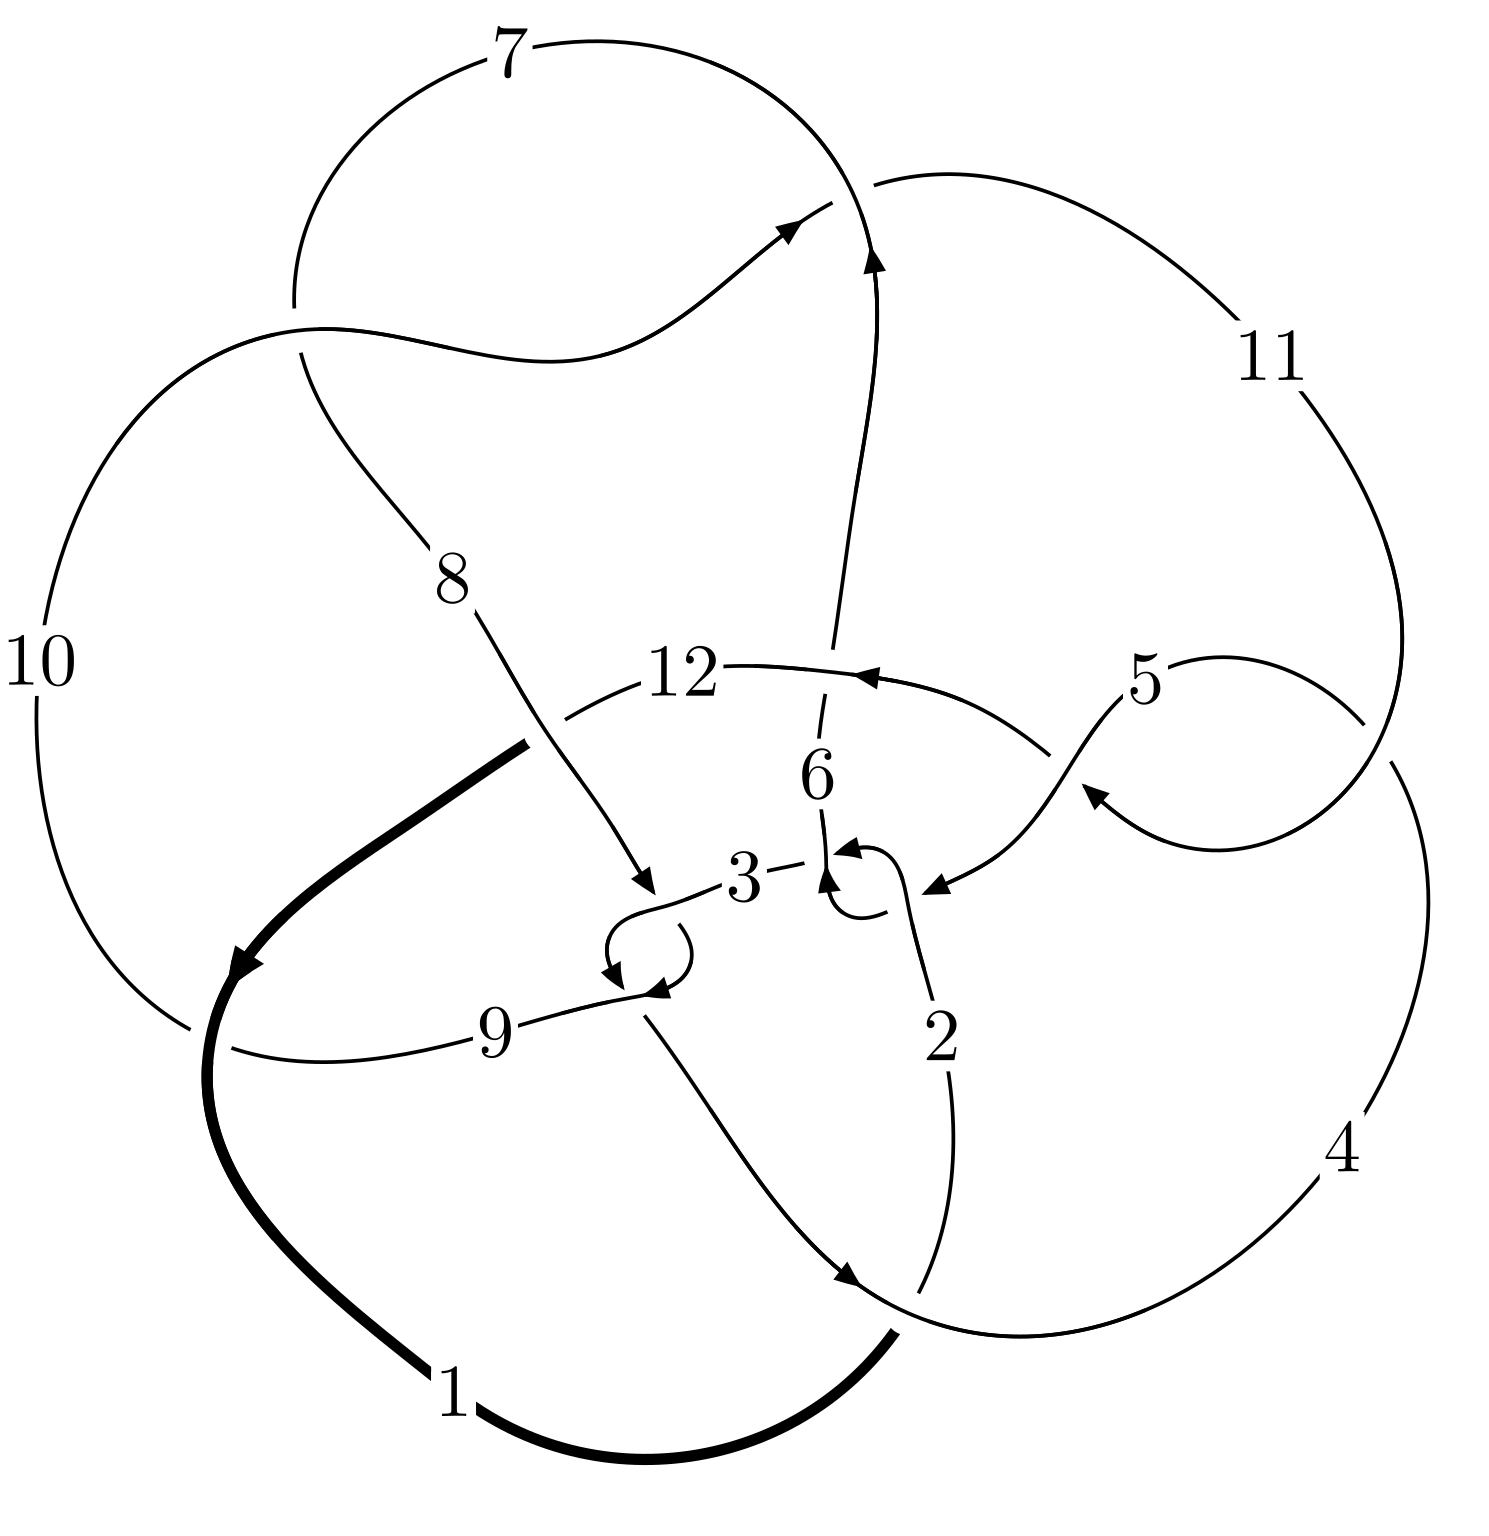
\includegraphics[width=112pt]{../../../GIT/diagram.site/Diagrams/png/1726_12a_0925.png}\\
\ \ \ A knot diagram\footnotemark}&
\allowdisplaybreaks
\textbf{Linearized knot diagam} \\
\cline{2-2}
 &
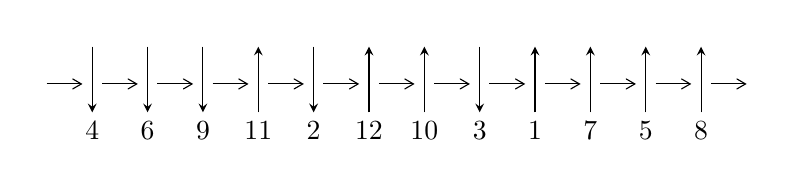
\begin{tikzpicture}[x=20pt, y=17pt]
	% nodes
	\node (C0) at (0, 0) {};
	\node (C1) at (1, 0) {};
	\node (C1U) at (1, +1) {};
	\node (C1D) at (1, -1) {4};

	\node (C2) at (2, 0) {};
	\node (C2U) at (2, +1) {};
	\node (C2D) at (2, -1) {6};

	\node (C3) at (3, 0) {};
	\node (C3U) at (3, +1) {};
	\node (C3D) at (3, -1) {9};

	\node (C4) at (4, 0) {};
	\node (C4U) at (4, +1) {};
	\node (C4D) at (4, -1) {11};

	\node (C5) at (5, 0) {};
	\node (C5U) at (5, +1) {};
	\node (C5D) at (5, -1) {2};

	\node (C6) at (6, 0) {};
	\node (C6U) at (6, +1) {};
	\node (C6D) at (6, -1) {12};

	\node (C7) at (7, 0) {};
	\node (C7U) at (7, +1) {};
	\node (C7D) at (7, -1) {10};

	\node (C8) at (8, 0) {};
	\node (C8U) at (8, +1) {};
	\node (C8D) at (8, -1) {3};

	\node (C9) at (9, 0) {};
	\node (C9U) at (9, +1) {};
	\node (C9D) at (9, -1) {1};

	\node (C10) at (10, 0) {};
	\node (C10U) at (10, +1) {};
	\node (C10D) at (10, -1) {7};

	\node (C11) at (11, 0) {};
	\node (C11U) at (11, +1) {};
	\node (C11D) at (11, -1) {5};

	\node (C12) at (12, 0) {};
	\node (C12U) at (12, +1) {};
	\node (C12D) at (12, -1) {8};
	\node (C13) at (13, 0) {};

	% arrows
	\draw[->,>={angle 60}]
	(C0) edge (C1) (C1) edge (C2) (C2) edge (C3) (C3) edge (C4) (C4) edge (C5) (C5) edge (C6) (C6) edge (C7) (C7) edge (C8) (C8) edge (C9) (C9) edge (C10) (C10) edge (C11) (C11) edge (C12) (C12) edge (C13) ;	\draw[->,>=stealth]
	(C1U) edge (C1D) (C2U) edge (C2D) (C3U) edge (C3D) (C4D) edge (C4U) (C5U) edge (C5D) (C6D) edge (C6U) (C7D) edge (C7U) (C8U) edge (C8D) (C9D) edge (C9U) (C10D) edge (C10U) (C11D) edge (C11U) (C12D) edge (C12U) ;
	\end{tikzpicture} \\
\hhline{~~} \\& 
\textbf{Solving Sequence} \\ \cline{2-2} 
 &
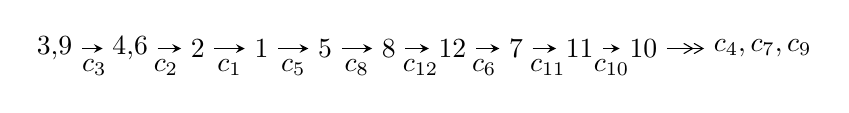
\begin{tikzpicture}[x=23pt, y=7pt]
	% node
	\node (A0) at (-1/8, 0) {3,9};
	\node (A1) at (17/16, 0) {4,6};
	\node (A2) at (17/8, 0) {2};
	\node (A3) at (25/8, 0) {1};
	\node (A4) at (33/8, 0) {5};
	\node (A5) at (41/8, 0) {8};
	\node (A6) at (49/8, 0) {12};
	\node (A7) at (57/8, 0) {7};
	\node (A8) at (65/8, 0) {11};
	\node (A9) at (73/8, 0) {10};
	\node (C1) at (1/2, -1) {$c_{3}$};
	\node (C2) at (13/8, -1) {$c_{2}$};
	\node (C3) at (21/8, -1) {$c_{1}$};
	\node (C4) at (29/8, -1) {$c_{5}$};
	\node (C5) at (37/8, -1) {$c_{8}$};
	\node (C6) at (45/8, -1) {$c_{12}$};
	\node (C7) at (53/8, -1) {$c_{6}$};
	\node (C8) at (61/8, -1) {$c_{11}$};
	\node (C9) at (69/8, -1) {$c_{10}$};
	\node (A10) at (11, 0) {$c_{4},c_{7},c_{9}$};

	% edge
	\draw[->,>=stealth]	
	(A0) edge (A1) (A1) edge (A2) (A2) edge (A3) (A3) edge (A4) (A4) edge (A5) (A5) edge (A6) (A6) edge (A7) (A7) edge (A8) (A8) edge (A9) ;
	\draw[->>,>={angle 60}]	
	(A9) edge (A10);
\end{tikzpicture} \\ 

\end{tabular} \\

\footnotetext{
The image of knot diagram is generated by the software ``\textbf{Draw programme}" developed by Andrew Bartholomew(\url{http://www.layer8.co.uk/maths/draw/index.htm\#Running-draw}), where we modified some parts for our purpose(\url{https://github.com/CATsTAILs/LinksPainter}).
}\phantom \\ \newline 
\centering \textbf{Ideals for irreducible components\footnotemark of $X_{\text{par}}$} 
 
\begin{align*}
I^u_{1}&=\langle 
-6.37208\times10^{955} u^{174}-5.29428\times10^{954} u^{173}+\cdots+1.52887\times10^{955} b+1.80446\times10^{959},\\
\phantom{I^u_{1}}&\phantom{= \langle  }-6.40167\times10^{959} u^{174}-5.34264\times10^{958} u^{173}+\cdots+4.00718\times10^{958} a+1.81672\times10^{963},\\
\phantom{I^u_{1}}&\phantom{= \langle  }u^{175}+u^{174}+\cdots-2853 u-2621\rangle \\
I^u_{2}&=\langle 
3.32259\times10^{40} u^{52}-2.34870\times10^{40} u^{51}+\cdots+1.43120\times10^{38} b+4.37472\times10^{40},\\
\phantom{I^u_{2}}&\phantom{= \langle  }-1.47911\times10^{41} u^{52}+8.39026\times10^{40} u^{51}+\cdots+1.43120\times10^{38} a-1.72574\times10^{41},\\
\phantom{I^u_{2}}&\phantom{= \langle  }u^{53}-14 u^{51}+\cdots-11 u^2+1\rangle \\
\\
\end{align*}
\raggedright * 2 irreducible components of $\dim_{\mathbb{C}}=0$, with total 228 representations.\\
\footnotetext{All coefficients of polynomials are rational numbers. But the coefficients are sometimes approximated in decimal forms when there is not enough margin.}
\newpage
\renewcommand{\arraystretch}{1}
\centering \section*{I. $I^u_{1}= \langle -6.37\times10^{955} u^{174}-5.29\times10^{954} u^{173}+\cdots+1.53\times10^{955} b+1.80\times10^{959},\;-6.40\times10^{959} u^{174}-5.34\times10^{958} u^{173}+\cdots+4.01\times10^{958} a+1.82\times10^{963},\;u^{175}+u^{174}+\cdots-2853 u-2621 \rangle$}
\flushleft \textbf{(i) Arc colorings}\\
\begin{tabular}{m{7pt} m{180pt} m{7pt} m{180pt} }
\flushright $a_{3}=$&$\begin{pmatrix}1\\0\end{pmatrix}$ \\
\flushright $a_{9}=$&$\begin{pmatrix}0\\u\end{pmatrix}$ \\
\flushright $a_{4}=$&$\begin{pmatrix}1\\u^2\end{pmatrix}$ \\
\flushright $a_{6}=$&$\begin{pmatrix}15.9755 u^{174}+1.33327 u^{173}+\cdots-36.3411 u-45336.5\\4.16783 u^{174}+0.346286 u^{173}+\cdots-35.5749 u-11802.5\end{pmatrix}$ \\
\flushright $a_{2}=$&$\begin{pmatrix}-7.11073 u^{174}-0.574352 u^{173}+\cdots-66.0517 u+20079.5\\-0.176273 u^{174}+0.265217 u^{173}+\cdots+849.646 u-407.719\end{pmatrix}$ \\
\flushright $a_{1}=$&$\begin{pmatrix}-1.19707 u^{174}+0.161818 u^{173}+\cdots+772.531 u+2539.92\\4.37966 u^{174}+0.848427 u^{173}+\cdots+1577.97 u-13977.9\end{pmatrix}$ \\
\flushright $a_{5}=$&$\begin{pmatrix}13.0539 u^{174}+0.606725 u^{173}+\cdots-1662.11 u-35463.6\\9.15087 u^{174}+0.394872 u^{173}+\cdots-1353.36 u-24800.8\end{pmatrix}$ \\
\flushright $a_{8}=$&$\begin{pmatrix}u\\u\end{pmatrix}$ \\
\flushright $a_{12}=$&$\begin{pmatrix}-5.51568 u^{174}-0.379165 u^{173}+\cdots+107.438 u+15356.9\\0.0610535 u^{174}+0.307444 u^{173}+\cdots+912.877 u-1160.90\end{pmatrix}$ \\
\flushright $a_{7}=$&$\begin{pmatrix}1.37797 u^{174}-0.870688 u^{173}+\cdots-3364.65 u-674.753\\5.18568 u^{174}-0.184804 u^{173}+\cdots-2096.15 u-12781.4\end{pmatrix}$ \\
\flushright $a_{11}=$&$\begin{pmatrix}-0.476362 u^{174}+0.160489 u^{173}+\cdots+766.812 u+911.061\\-6.49332 u^{174}-0.319529 u^{173}+\cdots+879.629 u+17886.6\end{pmatrix}$ \\
\flushright $a_{10}=$&$\begin{pmatrix}-13.6307 u^{174}-1.30945 u^{173}+\cdots-209.392 u+39302.5\\-7.00162 u^{174}-0.711508 u^{173}+\cdots-27.9154 u+20160.6\end{pmatrix}$\\&\end{tabular}
\flushleft \textbf{(ii) Obstruction class $= -1$}\\~\\
\flushleft \textbf{(iii) Cusp Shapes $= -32.4777 u^{174}-3.37563 u^{173}+\cdots-2284.15 u+94315.5$}\\~\\
\newpage\renewcommand{\arraystretch}{1}
\flushleft \textbf{(iv) u-Polynomials at the component}\newline \\
\begin{tabular}{m{50pt}|m{274pt}}
Crossings & \hspace{64pt}u-Polynomials at each crossing \\
\hline $$\begin{aligned}c_{1}\end{aligned}$$&$\begin{aligned}
&u^{175}-8 u^{174}+\cdots+1890868908462 u-280537441299
\end{aligned}$\\
\hline $$\begin{aligned}c_{2},c_{5}\end{aligned}$$&$\begin{aligned}
&u^{175}+4 u^{174}+\cdots+417270 u+63403
\end{aligned}$\\
\hline $$\begin{aligned}c_{3},c_{8}\end{aligned}$$&$\begin{aligned}
&u^{175}+u^{174}+\cdots-2853 u-2621
\end{aligned}$\\
\hline $$\begin{aligned}c_{4},c_{11}\end{aligned}$$&$\begin{aligned}
&u^{175}+u^{174}+\cdots-21401 u+1549
\end{aligned}$\\
\hline $$\begin{aligned}c_{6}\end{aligned}$$&$\begin{aligned}
&u^{175}-2 u^{174}+\cdots-657105 u+475777
\end{aligned}$\\
\hline $$\begin{aligned}c_{7},c_{10}\end{aligned}$$&$\begin{aligned}
&u^{175}+6 u^{174}+\cdots-343340 u-23572
\end{aligned}$\\
\hline $$\begin{aligned}c_{9}\end{aligned}$$&$\begin{aligned}
&u^{175}-6 u^{174}+\cdots+4627516764 u+594875704
\end{aligned}$\\
\hline $$\begin{aligned}c_{12}\end{aligned}$$&$\begin{aligned}
&u^{175}+2 u^{174}+\cdots-218568 u+5697
\end{aligned}$\\
\hline
\end{tabular}\\~\\
\newpage\renewcommand{\arraystretch}{1}
\flushleft \textbf{(v) Riley Polynomials at the component}\newline \\
\begin{tabular}{m{50pt}|m{274pt}}
Crossings & \hspace{64pt}Riley Polynomials at each crossing \\
\hline $$\begin{aligned}c_{1}\end{aligned}$$&$\begin{aligned}
&y^{175}-52 y^{174}+\cdots+3.27\times10^{24} y-7.87\times10^{22}
\end{aligned}$\\
\hline $$\begin{aligned}c_{2},c_{5}\end{aligned}$$&$\begin{aligned}
&y^{175}-96 y^{174}+\cdots+241757138316 y-4019940409
\end{aligned}$\\
\hline $$\begin{aligned}c_{3},c_{8}\end{aligned}$$&$\begin{aligned}
&y^{175}-107 y^{174}+\cdots+304239221 y-6869641
\end{aligned}$\\
\hline $$\begin{aligned}c_{4},c_{11}\end{aligned}$$&$\begin{aligned}
&y^{175}-87 y^{174}+\cdots+251496317 y-2399401
\end{aligned}$\\
\hline $$\begin{aligned}c_{6}\end{aligned}$$&$\begin{aligned}
&y^{175}+18 y^{174}+\cdots-12874725123895 y-226363753729
\end{aligned}$\\
\hline $$\begin{aligned}c_{7},c_{10}\end{aligned}$$&$\begin{aligned}
&y^{175}+122 y^{174}+\cdots-6061106160 y-555639184
\end{aligned}$\\
\hline $$\begin{aligned}c_{9}\end{aligned}$$&$\begin{aligned}
&y^{175}+62 y^{174}+\cdots-2.61\times10^{19} y-3.54\times10^{17}
\end{aligned}$\\
\hline $$\begin{aligned}c_{12}\end{aligned}$$&$\begin{aligned}
&y^{175}+62 y^{174}+\cdots-12813231636 y-32455809
\end{aligned}$\\
\hline
\end{tabular}\\~\\
\newpage\flushleft \textbf{(vi) Complex Volumes and Cusp Shapes}
$$\begin{array}{c|c|c}  
\text{Solutions to }I^u_{1}& \I (\text{vol} + \sqrt{-1}CS) & \text{Cusp shape}\\
 \hline 
\begin{aligned}
u &= -1.008340 + 0.114977 I \\
a &= \phantom{-}0.06770 + 2.00673 I \\
b &= -0.639902 - 0.509941 I\end{aligned}
 & -0.72811 + 5.24649 I & \phantom{-0.000000 } 0 \\ \hline\begin{aligned}
u &= -1.008340 - 0.114977 I \\
a &= \phantom{-}0.06770 - 2.00673 I \\
b &= -0.639902 + 0.509941 I\end{aligned}
 & -0.72811 - 5.24649 I & \phantom{-0.000000 } 0 \\ \hline\begin{aligned}
u &= \phantom{-}0.052380 + 0.983705 I \\
a &= -0.271367 + 0.895018 I \\
b &= -0.175627 - 1.046830 I\end{aligned}
 & \phantom{-}0.09640 + 8.25979 I & \phantom{-0.000000 } 0 \\ \hline\begin{aligned}
u &= \phantom{-}0.052380 - 0.983705 I \\
a &= -0.271367 - 0.895018 I \\
b &= -0.175627 + 1.046830 I\end{aligned}
 & \phantom{-}0.09640 - 8.25979 I & \phantom{-0.000000 } 0 \\ \hline\begin{aligned}
u &= -0.969775 + 0.092941 I \\
a &= \phantom{-}0.404042 + 1.238470 I \\
b &= \phantom{-}0.56097 + 1.30163 I\end{aligned}
 & \phantom{-}0.779150 - 0.881346 I & \phantom{-0.000000 } 0 \\ \hline\begin{aligned}
u &= -0.969775 - 0.092941 I \\
a &= \phantom{-}0.404042 - 1.238470 I \\
b &= \phantom{-}0.56097 - 1.30163 I\end{aligned}
 & \phantom{-}0.779150 + 0.881346 I & \phantom{-0.000000 } 0 \\ \hline\begin{aligned}
u &= \phantom{-}0.894099 + 0.360744 I \\
a &= -0.117949 + 0.659180 I \\
b &= \phantom{-}0.740112 - 0.004916 I\end{aligned}
 & -6.23141 + 0.57035 I & \phantom{-0.000000 } 0 \\ \hline\begin{aligned}
u &= \phantom{-}0.894099 - 0.360744 I \\
a &= -0.117949 - 0.659180 I \\
b &= \phantom{-}0.740112 + 0.004916 I\end{aligned}
 & -6.23141 - 0.57035 I & \phantom{-0.000000 } 0 \\ \hline\begin{aligned}
u &= -0.731796 + 0.610840 I \\
a &= -0.568517 + 0.583153 I \\
b &= \phantom{-}1.120150 + 0.353376 I\end{aligned}
 & \phantom{-}1.57326 - 1.76025 I & \phantom{-0.000000 } 0 \\ \hline\begin{aligned}
u &= -0.731796 - 0.610840 I \\
a &= -0.568517 - 0.583153 I \\
b &= \phantom{-}1.120150 - 0.353376 I\end{aligned}
 & \phantom{-}1.57326 + 1.76025 I & \phantom{-0.000000 } 0\\
 \hline 
 \end{array}$$\newpage$$\begin{array}{c|c|c}  
\text{Solutions to }I^u_{1}& \I (\text{vol} + \sqrt{-1}CS) & \text{Cusp shape}\\
 \hline 
\begin{aligned}
u &= \phantom{-}0.918709 + 0.237229 I \\
a &= \phantom{-}0.270110 - 0.894702 I \\
b &= -0.536386 + 0.661275 I\end{aligned}
 & \phantom{-}2.86322 - 1.32931 I & \phantom{-0.000000 } 0 \\ \hline\begin{aligned}
u &= \phantom{-}0.918709 - 0.237229 I \\
a &= \phantom{-}0.270110 + 0.894702 I \\
b &= -0.536386 - 0.661275 I\end{aligned}
 & \phantom{-}2.86322 + 1.32931 I & \phantom{-0.000000 } 0 \\ \hline\begin{aligned}
u &= \phantom{-}1.055870 + 0.100541 I \\
a &= -0.402174 + 0.029672 I \\
b &= \phantom{-}0.529728 + 0.479846 I\end{aligned}
 & -6.48509 + 0.71958 I & \phantom{-0.000000 } 0 \\ \hline\begin{aligned}
u &= \phantom{-}1.055870 - 0.100541 I \\
a &= -0.402174 - 0.029672 I \\
b &= \phantom{-}0.529728 - 0.479846 I\end{aligned}
 & -6.48509 - 0.71958 I & \phantom{-0.000000 } 0 \\ \hline\begin{aligned}
u &= -1.058450 + 0.124315 I \\
a &= -2.55497 - 0.49443 I \\
b &= -1.283910 + 0.415138 I\end{aligned}
 & -3.02613 + 1.59757 I & \phantom{-0.000000 } 0 \\ \hline\begin{aligned}
u &= -1.058450 - 0.124315 I \\
a &= -2.55497 + 0.49443 I \\
b &= -1.283910 - 0.415138 I\end{aligned}
 & -3.02613 - 1.59757 I & \phantom{-0.000000 } 0 \\ \hline\begin{aligned}
u &= -0.923940 + 0.062597 I \\
a &= -1.118240 + 0.104649 I \\
b &= -0.819568 + 1.135490 I\end{aligned}
 & \phantom{-}0.99939 + 1.70499 I & \phantom{-0.000000 } 0 \\ \hline\begin{aligned}
u &= -0.923940 - 0.062597 I \\
a &= -1.118240 - 0.104649 I \\
b &= -0.819568 - 1.135490 I\end{aligned}
 & \phantom{-}0.99939 - 1.70499 I & \phantom{-0.000000 } 0 \\ \hline\begin{aligned}
u &= -0.815324 + 0.429136 I \\
a &= -0.19301 - 1.45744 I \\
b &= -1.034920 + 0.535439 I\end{aligned}
 & \phantom{-}1.35633 + 5.98085 I & \phantom{-0.000000 } 0 \\ \hline\begin{aligned}
u &= -0.815324 - 0.429136 I \\
a &= -0.19301 + 1.45744 I \\
b &= -1.034920 - 0.535439 I\end{aligned}
 & \phantom{-}1.35633 - 5.98085 I & \phantom{-0.000000 } 0\\
 \hline 
 \end{array}$$\newpage$$\begin{array}{c|c|c}  
\text{Solutions to }I^u_{1}& \I (\text{vol} + \sqrt{-1}CS) & \text{Cusp shape}\\
 \hline 
\begin{aligned}
u &= \phantom{-}0.912619 + 0.122850 I \\
a &= -0.227881 - 1.307120 I \\
b &= -0.102478 - 1.254120 I\end{aligned}
 & \phantom{-}1.44152 - 3.97683 I & \phantom{-0.000000 } 0 \\ \hline\begin{aligned}
u &= \phantom{-}0.912619 - 0.122850 I \\
a &= -0.227881 + 1.307120 I \\
b &= -0.102478 + 1.254120 I\end{aligned}
 & \phantom{-}1.44152 + 3.97683 I & \phantom{-0.000000 } 0 \\ \hline\begin{aligned}
u &= \phantom{-}0.857554 + 0.331513 I \\
a &= \phantom{-}0.75497 + 1.63777 I \\
b &= -1.030800 - 0.444653 I\end{aligned}
 & -1.97267 - 9.14333 I & \phantom{-0.000000 } 0 \\ \hline\begin{aligned}
u &= \phantom{-}0.857554 - 0.331513 I \\
a &= \phantom{-}0.75497 - 1.63777 I \\
b &= -1.030800 + 0.444653 I\end{aligned}
 & -1.97267 + 9.14333 I & \phantom{-0.000000 } 0 \\ \hline\begin{aligned}
u &= \phantom{-}0.766214 + 0.499618 I \\
a &= -0.91660 - 1.50789 I \\
b &= \phantom{-}1.133460 - 0.201915 I\end{aligned}
 & -1.82975 + 5.58360 I & \phantom{-0.000000 } 0 \\ \hline\begin{aligned}
u &= \phantom{-}0.766214 - 0.499618 I \\
a &= -0.91660 + 1.50789 I \\
b &= \phantom{-}1.133460 + 0.201915 I\end{aligned}
 & -1.82975 - 5.58360 I & \phantom{-0.000000 } 0 \\ \hline\begin{aligned}
u &= -0.681198 + 0.607884 I \\
a &= \phantom{-}0.341632 + 0.617565 I \\
b &= \phantom{-}0.713431 + 0.601410 I\end{aligned}
 & -1.43546 - 3.18285 I & \phantom{-0.000000 } 0 \\ \hline\begin{aligned}
u &= -0.681198 - 0.607884 I \\
a &= \phantom{-}0.341632 - 0.617565 I \\
b &= \phantom{-}0.713431 - 0.601410 I\end{aligned}
 & -1.43546 + 3.18285 I & \phantom{-0.000000 } 0 \\ \hline\begin{aligned}
u &= \phantom{-}1.055600 + 0.262250 I \\
a &= -2.41064 + 0.62625 I \\
b &= -1.359230 - 0.365500 I\end{aligned}
 & -6.00895 - 5.26943 I & \phantom{-0.000000 } 0 \\ \hline\begin{aligned}
u &= \phantom{-}1.055600 - 0.262250 I \\
a &= -2.41064 - 0.62625 I \\
b &= -1.359230 + 0.365500 I\end{aligned}
 & -6.00895 + 5.26943 I & \phantom{-0.000000 } 0\\
 \hline 
 \end{array}$$\newpage$$\begin{array}{c|c|c}  
\text{Solutions to }I^u_{1}& \I (\text{vol} + \sqrt{-1}CS) & \text{Cusp shape}\\
 \hline 
\begin{aligned}
u &= \phantom{-}0.983587 + 0.477897 I \\
a &= \phantom{-}1.267250 - 0.165255 I \\
b &= \phantom{-}0.727556 + 0.809995 I\end{aligned}
 & -1.49248 - 2.13116 I & \phantom{-0.000000 } 0 \\ \hline\begin{aligned}
u &= \phantom{-}0.983587 - 0.477897 I \\
a &= \phantom{-}1.267250 + 0.165255 I \\
b &= \phantom{-}0.727556 - 0.809995 I\end{aligned}
 & -1.49248 + 2.13116 I & \phantom{-0.000000 } 0 \\ \hline\begin{aligned}
u &= -0.890066 + 0.167770 I \\
a &= \phantom{-}0.478732 + 0.037537 I \\
b &= \phantom{-}0.565199 - 0.581016 I\end{aligned}
 & -1.47170 + 0.87487 I & \phantom{-0.000000 } 0 \\ \hline\begin{aligned}
u &= -0.890066 - 0.167770 I \\
a &= \phantom{-}0.478732 - 0.037537 I \\
b &= \phantom{-}0.565199 + 0.581016 I\end{aligned}
 & -1.47170 - 0.87487 I & \phantom{-0.000000 } 0 \\ \hline\begin{aligned}
u &= \phantom{-}0.750069 + 0.798108 I \\
a &= \phantom{-}0.599263 - 0.776735 I \\
b &= \phantom{-}0.714467 - 0.072197 I\end{aligned}
 & \phantom{-}0.409841 + 0.584531 I & \phantom{-0.000000 } 0 \\ \hline\begin{aligned}
u &= \phantom{-}0.750069 - 0.798108 I \\
a &= \phantom{-}0.599263 + 0.776735 I \\
b &= \phantom{-}0.714467 + 0.072197 I\end{aligned}
 & \phantom{-}0.409841 - 0.584531 I & \phantom{-0.000000 } 0 \\ \hline\begin{aligned}
u &= \phantom{-}1.110910 + 0.016667 I \\
a &= -2.93249 + 0.41183 I \\
b &= -1.149250 - 0.374540 I\end{aligned}
 & -7.32014 + 1.45894 I & \phantom{-0.000000 } 0 \\ \hline\begin{aligned}
u &= \phantom{-}1.110910 - 0.016667 I \\
a &= -2.93249 - 0.41183 I \\
b &= -1.149250 + 0.374540 I\end{aligned}
 & -7.32014 - 1.45894 I & \phantom{-0.000000 } 0 \\ \hline\begin{aligned}
u &= -0.885283 + 0.024542 I \\
a &= \phantom{-}4.60948 - 1.59603 I \\
b &= \phantom{-}0.758385 - 0.020744 I\end{aligned}
 & -0.05882 - 4.46982 I & \phantom{-0.000000 } 0 \\ \hline\begin{aligned}
u &= -0.885283 - 0.024542 I \\
a &= \phantom{-}4.60948 + 1.59603 I \\
b &= \phantom{-}0.758385 + 0.020744 I\end{aligned}
 & -0.05882 + 4.46982 I & \phantom{-0.000000 } 0\\
 \hline 
 \end{array}$$\newpage$$\begin{array}{c|c|c}  
\text{Solutions to }I^u_{1}& \I (\text{vol} + \sqrt{-1}CS) & \text{Cusp shape}\\
 \hline 
\begin{aligned}
u &= -1.077380 + 0.293356 I \\
a &= \phantom{-}2.45114 + 0.40387 I \\
b &= \phantom{-}1.48414 - 0.56183 I\end{aligned}
 & -3.80384 + 10.36360 I & \phantom{-0.000000 } 0 \\ \hline\begin{aligned}
u &= -1.077380 - 0.293356 I \\
a &= \phantom{-}2.45114 - 0.40387 I \\
b &= \phantom{-}1.48414 + 0.56183 I\end{aligned}
 & -3.80384 - 10.36360 I & \phantom{-0.000000 } 0 \\ \hline\begin{aligned}
u &= \phantom{-}0.882540\phantom{ +0.000000I} \\
a &= \phantom{-}4.88625\phantom{ +0.000000I} \\
b &= \phantom{-}0.757507\phantom{ +0.000000I}\end{aligned}
 & \phantom{-}3.90842\phantom{ +0.000000I} & \phantom{-0.000000 } 0 \\ \hline\begin{aligned}
u &= -1.061440 + 0.363688 I \\
a &= \phantom{-}1.55159 + 0.32538 I \\
b &= \phantom{-}0.917976 - 0.612189 I\end{aligned}
 & -1.40636 + 2.81522 I & \phantom{-0.000000 } 0 \\ \hline\begin{aligned}
u &= -1.061440 - 0.363688 I \\
a &= \phantom{-}1.55159 - 0.32538 I \\
b &= \phantom{-}0.917976 + 0.612189 I\end{aligned}
 & -1.40636 - 2.81522 I & \phantom{-0.000000 } 0 \\ \hline\begin{aligned}
u &= \phantom{-}1.104410 + 0.224190 I \\
a &= \phantom{-}2.09979 - 0.37926 I \\
b &= \phantom{-}1.30053 + 0.77145 I\end{aligned}
 & -1.80068 - 6.55713 I & \phantom{-0.000000 } 0 \\ \hline\begin{aligned}
u &= \phantom{-}1.104410 - 0.224190 I \\
a &= \phantom{-}2.09979 + 0.37926 I \\
b &= \phantom{-}1.30053 - 0.77145 I\end{aligned}
 & -1.80068 + 6.55713 I & \phantom{-0.000000 } 0 \\ \hline\begin{aligned}
u &= \phantom{-}0.313944 + 0.808747 I \\
a &= \phantom{-}0.103102 + 0.433947 I \\
b &= -0.850043 - 0.444944 I\end{aligned}
 & \phantom{-}1.81980 + 0.11582 I & \phantom{-0.000000 } 0 \\ \hline\begin{aligned}
u &= \phantom{-}0.313944 - 0.808747 I \\
a &= \phantom{-}0.103102 - 0.433947 I \\
b &= -0.850043 + 0.444944 I\end{aligned}
 & \phantom{-}1.81980 - 0.11582 I & \phantom{-0.000000 } 0 \\ \hline\begin{aligned}
u &= -1.126140 + 0.168539 I \\
a &= \phantom{-}1.54899 + 1.33006 I \\
b &= \phantom{-}0.986495 - 0.615170 I\end{aligned}
 & -7.60050 + 5.26863 I & \phantom{-0.000000 } 0\\
 \hline 
 \end{array}$$\newpage$$\begin{array}{c|c|c}  
\text{Solutions to }I^u_{1}& \I (\text{vol} + \sqrt{-1}CS) & \text{Cusp shape}\\
 \hline 
\begin{aligned}
u &= -1.126140 - 0.168539 I \\
a &= \phantom{-}1.54899 - 1.33006 I \\
b &= \phantom{-}0.986495 + 0.615170 I\end{aligned}
 & -7.60050 - 5.26863 I & \phantom{-0.000000 } 0 \\ \hline\begin{aligned}
u &= \phantom{-}1.101550 + 0.327879 I \\
a &= \phantom{-}0.601592 - 0.264941 I \\
b &= \phantom{-}0.463340 + 0.801709 I\end{aligned}
 & -1.11431 - 4.04608 I & \phantom{-0.000000 } 0 \\ \hline\begin{aligned}
u &= \phantom{-}1.101550 - 0.327879 I \\
a &= \phantom{-}0.601592 + 0.264941 I \\
b &= \phantom{-}0.463340 - 0.801709 I\end{aligned}
 & -1.11431 + 4.04608 I & \phantom{-0.000000 } 0 \\ \hline\begin{aligned}
u &= \phantom{-}0.294355 + 1.111750 I \\
a &= \phantom{-}0.089913 + 0.361865 I \\
b &= \phantom{-}1.46643 - 0.36244 I\end{aligned}
 & -5.19682 - 3.12832 I & \phantom{-0.000000 } 0 \\ \hline\begin{aligned}
u &= \phantom{-}0.294355 - 1.111750 I \\
a &= \phantom{-}0.089913 - 0.361865 I \\
b &= \phantom{-}1.46643 + 0.36244 I\end{aligned}
 & -5.19682 + 3.12832 I & \phantom{-0.000000 } 0 \\ \hline\begin{aligned}
u &= -0.555505 + 1.007470 I \\
a &= \phantom{-}0.056272 + 0.654668 I \\
b &= -1.065360 - 0.663216 I\end{aligned}
 & -4.41497 - 0.27045 I & \phantom{-0.000000 } 0 \\ \hline\begin{aligned}
u &= -0.555505 - 1.007470 I \\
a &= \phantom{-}0.056272 - 0.654668 I \\
b &= -1.065360 + 0.663216 I\end{aligned}
 & -4.41497 + 0.27045 I & \phantom{-0.000000 } 0 \\ \hline\begin{aligned}
u &= -1.050050 + 0.493222 I \\
a &= -0.510811 + 0.751441 I \\
b &= \phantom{-}0.648656 - 0.018944 I\end{aligned}
 & -5.54541 + 6.77031 I & \phantom{-0.000000 } 0 \\ \hline\begin{aligned}
u &= -1.050050 - 0.493222 I \\
a &= -0.510811 - 0.751441 I \\
b &= \phantom{-}0.648656 + 0.018944 I\end{aligned}
 & -5.54541 - 6.77031 I & \phantom{-0.000000 } 0 \\ \hline\begin{aligned}
u &= \phantom{-}1.061500 + 0.473801 I \\
a &= -0.148639 - 0.686284 I \\
b &= \phantom{-}0.394648 - 0.169968 I\end{aligned}
 & -0.57205 - 4.46548 I & \phantom{-0.000000 } 0\\
 \hline 
 \end{array}$$\newpage$$\begin{array}{c|c|c}  
\text{Solutions to }I^u_{1}& \I (\text{vol} + \sqrt{-1}CS) & \text{Cusp shape}\\
 \hline 
\begin{aligned}
u &= \phantom{-}1.061500 - 0.473801 I \\
a &= -0.148639 + 0.686284 I \\
b &= \phantom{-}0.394648 + 0.169968 I\end{aligned}
 & -0.57205 + 4.46548 I & \phantom{-0.000000 } 0 \\ \hline\begin{aligned}
u &= -0.130560 + 0.823512 I \\
a &= \phantom{-}0.590084 + 0.629492 I \\
b &= \phantom{-}0.096768 - 0.484498 I\end{aligned}
 & -2.76466 - 3.57057 I & \phantom{-0.000000 } 0 \\ \hline\begin{aligned}
u &= -0.130560 - 0.823512 I \\
a &= \phantom{-}0.590084 - 0.629492 I \\
b &= \phantom{-}0.096768 + 0.484498 I\end{aligned}
 & -2.76466 + 3.57057 I & \phantom{-0.000000 } 0 \\ \hline\begin{aligned}
u &= \phantom{-}0.140766 + 0.807970 I \\
a &= -0.59109 - 1.62492 I \\
b &= -0.088000 + 0.863080 I\end{aligned}
 & \phantom{-}5.30870 - 1.78531 I & \phantom{-0.000000 } 0 \\ \hline\begin{aligned}
u &= \phantom{-}0.140766 - 0.807970 I \\
a &= -0.59109 + 1.62492 I \\
b &= -0.088000 - 0.863080 I\end{aligned}
 & \phantom{-}5.30870 + 1.78531 I & \phantom{-0.000000 } 0 \\ \hline\begin{aligned}
u &= -0.148594 + 1.173010 I \\
a &= -0.407767 + 0.518930 I \\
b &= -1.282450 - 0.593367 I\end{aligned}
 & -3.3301 - 14.1176 I & \phantom{-0.000000 } 0 \\ \hline\begin{aligned}
u &= -0.148594 - 1.173010 I \\
a &= -0.407767 - 0.518930 I \\
b &= -1.282450 + 0.593367 I\end{aligned}
 & -3.3301 + 14.1176 I & \phantom{-0.000000 } 0 \\ \hline\begin{aligned}
u &= -1.157350 + 0.257215 I \\
a &= -0.137219 + 0.951199 I \\
b &= \phantom{-}0.277699 + 0.698109 I\end{aligned}
 & -3.62656 + 4.64520 I & \phantom{-0.000000 } 0 \\ \hline\begin{aligned}
u &= -1.157350 - 0.257215 I \\
a &= -0.137219 - 0.951199 I \\
b &= \phantom{-}0.277699 - 0.698109 I\end{aligned}
 & -3.62656 - 4.64520 I & \phantom{-0.000000 } 0 \\ \hline\begin{aligned}
u &= \phantom{-}0.764638 + 0.280136 I \\
a &= -0.137922 - 0.343939 I \\
b &= -0.161390 - 0.992421 I\end{aligned}
 & \phantom{-}1.47080 + 1.90539 I & \phantom{-0.000000 } 0\\
 \hline 
 \end{array}$$\newpage$$\begin{array}{c|c|c}  
\text{Solutions to }I^u_{1}& \I (\text{vol} + \sqrt{-1}CS) & \text{Cusp shape}\\
 \hline 
\begin{aligned}
u &= \phantom{-}0.764638 - 0.280136 I \\
a &= -0.137922 + 0.343939 I \\
b &= -0.161390 + 0.992421 I\end{aligned}
 & \phantom{-}1.47080 - 1.90539 I & \phantom{-0.000000 } 0 \\ \hline\begin{aligned}
u &= \phantom{-}0.619257 + 0.514956 I \\
a &= -0.66997 + 1.96532 I \\
b &= -0.934962 - 0.523006 I\end{aligned}
 & -3.97045 - 4.40481 I & \phantom{-0.000000 } 0 \\ \hline\begin{aligned}
u &= \phantom{-}0.619257 - 0.514956 I \\
a &= -0.66997 - 1.96532 I \\
b &= -0.934962 + 0.523006 I\end{aligned}
 & -3.97045 + 4.40481 I & \phantom{-0.000000 } 0 \\ \hline\begin{aligned}
u &= -0.640063 + 0.469754 I \\
a &= -1.268060 - 0.484721 I \\
b &= -1.026780 + 0.705633 I\end{aligned}
 & -1.34087 + 7.56322 I & \phantom{-0.000000 } 0 \\ \hline\begin{aligned}
u &= -0.640063 - 0.469754 I \\
a &= -1.268060 + 0.484721 I \\
b &= -1.026780 - 0.705633 I\end{aligned}
 & -1.34087 - 7.56322 I & \phantom{-0.000000 } 0 \\ \hline\begin{aligned}
u &= \phantom{-}0.018313 + 0.788627 I \\
a &= \phantom{-}0.695905 + 0.160230 I \\
b &= \phantom{-}1.312860 + 0.110976 I\end{aligned}
 & -5.42053 - 0.73784 I & \phantom{-0.000000 } 0 \\ \hline\begin{aligned}
u &= \phantom{-}0.018313 - 0.788627 I \\
a &= \phantom{-}0.695905 - 0.160230 I \\
b &= \phantom{-}1.312860 - 0.110976 I\end{aligned}
 & -5.42053 + 0.73784 I & \phantom{-0.000000 } 0 \\ \hline\begin{aligned}
u &= \phantom{-}0.068963 + 1.210180 I \\
a &= \phantom{-}0.609750 + 0.396868 I \\
b &= \phantom{-}1.159300 - 0.409788 I\end{aligned}
 & -5.77869 + 7.27147 I & \phantom{-0.000000 } 0 \\ \hline\begin{aligned}
u &= \phantom{-}0.068963 - 1.210180 I \\
a &= \phantom{-}0.609750 - 0.396868 I \\
b &= \phantom{-}1.159300 + 0.409788 I\end{aligned}
 & -5.77869 - 7.27147 I & \phantom{-0.000000 } 0 \\ \hline\begin{aligned}
u &= \phantom{-}1.174220 + 0.406921 I \\
a &= \phantom{-}2.56128 - 0.72573 I \\
b &= \phantom{-}1.227910 + 0.245565 I\end{aligned}
 & -8.17152 - 7.99853 I & \phantom{-0.000000 } 0\\
 \hline 
 \end{array}$$\newpage$$\begin{array}{c|c|c}  
\text{Solutions to }I^u_{1}& \I (\text{vol} + \sqrt{-1}CS) & \text{Cusp shape}\\
 \hline 
\begin{aligned}
u &= \phantom{-}1.174220 - 0.406921 I \\
a &= \phantom{-}2.56128 + 0.72573 I \\
b &= \phantom{-}1.227910 - 0.245565 I\end{aligned}
 & -8.17152 + 7.99853 I & \phantom{-0.000000 } 0 \\ \hline\begin{aligned}
u &= -0.245489 + 1.220510 I \\
a &= \phantom{-}0.554382 - 0.267502 I \\
b &= \phantom{-}1.155370 + 0.256181 I\end{aligned}
 & -1.92129 - 1.96501 I & \phantom{-0.000000 } 0 \\ \hline\begin{aligned}
u &= -0.245489 - 1.220510 I \\
a &= \phantom{-}0.554382 + 0.267502 I \\
b &= \phantom{-}1.155370 - 0.256181 I\end{aligned}
 & -1.92129 + 1.96501 I & \phantom{-0.000000 } 0 \\ \hline\begin{aligned}
u &= -0.619235 + 0.424388 I \\
a &= \phantom{-}0.730260 - 0.027654 I \\
b &= \phantom{-}0.138368 - 0.650286 I\end{aligned}
 & -1.32344 + 1.75688 I & \phantom{-0.000000 } 0 \\ \hline\begin{aligned}
u &= -0.619235 - 0.424388 I \\
a &= \phantom{-}0.730260 + 0.027654 I \\
b &= \phantom{-}0.138368 + 0.650286 I\end{aligned}
 & -1.32344 - 1.75688 I & \phantom{-0.000000 } 0 \\ \hline\begin{aligned}
u &= -0.499157 + 0.558083 I \\
a &= \phantom{-}1.17487 - 0.96889 I \\
b &= -0.829562 + 0.095388 I\end{aligned}
 & -3.85851 - 2.55091 I & \phantom{-0.000000 } 0 \\ \hline\begin{aligned}
u &= -0.499157 - 0.558083 I \\
a &= \phantom{-}1.17487 + 0.96889 I \\
b &= -0.829562 - 0.095388 I\end{aligned}
 & -3.85851 + 2.55091 I & \phantom{-0.000000 } 0 \\ \hline\begin{aligned}
u &= -1.226400 + 0.318205 I \\
a &= \phantom{-}2.44179 + 0.60903 I \\
b &= \phantom{-}1.166520 - 0.436983 I\end{aligned}
 & -3.35407 + 7.74672 I & \phantom{-0.000000 } 0 \\ \hline\begin{aligned}
u &= -1.226400 - 0.318205 I \\
a &= \phantom{-}2.44179 - 0.60903 I \\
b &= \phantom{-}1.166520 + 0.436983 I\end{aligned}
 & -3.35407 - 7.74672 I & \phantom{-0.000000 } 0 \\ \hline\begin{aligned}
u &= -1.117490 + 0.599149 I \\
a &= \phantom{-}1.51665 + 1.46224 I \\
b &= \phantom{-}1.002940 - 0.072372 I\end{aligned}
 & -6.93585 + 0.03498 I & \phantom{-0.000000 } 0\\
 \hline 
 \end{array}$$\newpage$$\begin{array}{c|c|c}  
\text{Solutions to }I^u_{1}& \I (\text{vol} + \sqrt{-1}CS) & \text{Cusp shape}\\
 \hline 
\begin{aligned}
u &= -1.117490 - 0.599149 I \\
a &= \phantom{-}1.51665 - 1.46224 I \\
b &= \phantom{-}1.002940 + 0.072372 I\end{aligned}
 & -6.93585 - 0.03498 I & \phantom{-0.000000 } 0 \\ \hline\begin{aligned}
u &= \phantom{-}1.254460 + 0.223040 I \\
a &= \phantom{-}2.65308 - 0.66422 I \\
b &= \phantom{-}1.135600 + 0.530534 I\end{aligned}
 & -6.13100 - 9.36045 I & \phantom{-0.000000 } 0 \\ \hline\begin{aligned}
u &= \phantom{-}1.254460 - 0.223040 I \\
a &= \phantom{-}2.65308 + 0.66422 I \\
b &= \phantom{-}1.135600 - 0.530534 I\end{aligned}
 & -6.13100 + 9.36045 I & \phantom{-0.000000 } 0 \\ \hline\begin{aligned}
u &= -1.087070 + 0.683942 I \\
a &= \phantom{-}0.272679 + 0.266678 I \\
b &= \phantom{-}0.843710 + 0.265451 I\end{aligned}
 & \phantom{-}0.002842 + 1.006490 I & \phantom{-0.000000 } 0 \\ \hline\begin{aligned}
u &= -1.087070 - 0.683942 I \\
a &= \phantom{-}0.272679 - 0.266678 I \\
b &= \phantom{-}0.843710 - 0.265451 I\end{aligned}
 & \phantom{-}0.002842 - 1.006490 I & \phantom{-0.000000 } 0 \\ \hline\begin{aligned}
u &= \phantom{-}0.661990 + 0.268164 I \\
a &= -0.688289 - 0.333784 I \\
b &= -0.839786 - 0.696152 I\end{aligned}
 & \phantom{-}0.56526 - 5.07278 I & \phantom{-0.000000 } 0 \\ \hline\begin{aligned}
u &= \phantom{-}0.661990 - 0.268164 I \\
a &= -0.688289 + 0.333784 I \\
b &= -0.839786 + 0.696152 I\end{aligned}
 & \phantom{-}0.56526 + 5.07278 I & \phantom{-0.000000 } 0 \\ \hline\begin{aligned}
u &= \phantom{-}0.335407 + 1.244040 I \\
a &= -1.266040 - 0.155532 I \\
b &= -0.717952 + 0.021782 I\end{aligned}
 & \phantom{-}3.71341 - 3.52873 I & \phantom{-0.000000 } 0 \\ \hline\begin{aligned}
u &= \phantom{-}0.335407 - 1.244040 I \\
a &= -1.266040 + 0.155532 I \\
b &= -0.717952 - 0.021782 I\end{aligned}
 & \phantom{-}3.71341 + 3.52873 I & \phantom{-0.000000 } 0 \\ \hline\begin{aligned}
u &= \phantom{-}1.191900 + 0.500396 I \\
a &= \phantom{-}0.157852 - 0.714867 I \\
b &= \phantom{-}0.636888 - 0.475720 I\end{aligned}
 & -0.98080 - 4.93698 I & \phantom{-0.000000 } 0\\
 \hline 
 \end{array}$$\newpage$$\begin{array}{c|c|c}  
\text{Solutions to }I^u_{1}& \I (\text{vol} + \sqrt{-1}CS) & \text{Cusp shape}\\
 \hline 
\begin{aligned}
u &= \phantom{-}1.191900 - 0.500396 I \\
a &= \phantom{-}0.157852 + 0.714867 I \\
b &= \phantom{-}0.636888 + 0.475720 I\end{aligned}
 & -0.98080 + 4.93698 I & \phantom{-0.000000 } 0 \\ \hline\begin{aligned}
u &= -0.638722 + 1.126880 I \\
a &= -0.377501 - 0.675726 I \\
b &= -1.081380 + 0.332470 I\end{aligned}
 & \phantom{-}1.67900 + 5.40673 I & \phantom{-0.000000 } 0 \\ \hline\begin{aligned}
u &= -0.638722 - 1.126880 I \\
a &= -0.377501 + 0.675726 I \\
b &= -1.081380 - 0.332470 I\end{aligned}
 & \phantom{-}1.67900 - 5.40673 I & \phantom{-0.000000 } 0 \\ \hline\begin{aligned}
u &= \phantom{-}1.261520 + 0.301281 I \\
a &= \phantom{-}0.579930 + 0.064910 I \\
b &= \phantom{-}0.304684 + 1.160470 I\end{aligned}
 & -1.08964 - 3.91173 I & \phantom{-0.000000 } 0 \\ \hline\begin{aligned}
u &= \phantom{-}1.261520 - 0.301281 I \\
a &= \phantom{-}0.579930 - 0.064910 I \\
b &= \phantom{-}0.304684 - 1.160470 I\end{aligned}
 & -1.08964 + 3.91173 I & \phantom{-0.000000 } 0 \\ \hline\begin{aligned}
u &= -0.647164 + 0.262298 I \\
a &= \phantom{-}0.33760 + 1.75787 I \\
b &= -0.739546 + 0.278175 I\end{aligned}
 & -5.12039 + 4.35071 I & \phantom{-0.000000 } 0 \\ \hline\begin{aligned}
u &= -0.647164 - 0.262298 I \\
a &= \phantom{-}0.33760 - 1.75787 I \\
b &= -0.739546 - 0.278175 I\end{aligned}
 & -5.12039 - 4.35071 I & \phantom{-0.000000 } 0 \\ \hline\begin{aligned}
u &= -1.231500 + 0.453162 I \\
a &= -2.08904 - 0.92007 I \\
b &= -1.49855 + 0.17664 I\end{aligned}
 & -9.09985 + 5.23913 I & \phantom{-0.000000 } 0 \\ \hline\begin{aligned}
u &= -1.231500 - 0.453162 I \\
a &= -2.08904 + 0.92007 I \\
b &= -1.49855 - 0.17664 I\end{aligned}
 & -9.09985 - 5.23913 I & \phantom{-0.000000 } 0 \\ \hline\begin{aligned}
u &= \phantom{-}0.221710 + 1.307120 I \\
a &= -0.285676 - 0.469695 I \\
b &= -1.28686 + 0.60598 I\end{aligned}
 & \phantom{-}1.42759 + 7.54557 I & \phantom{-0.000000 } 0\\
 \hline 
 \end{array}$$\newpage$$\begin{array}{c|c|c}  
\text{Solutions to }I^u_{1}& \I (\text{vol} + \sqrt{-1}CS) & \text{Cusp shape}\\
 \hline 
\begin{aligned}
u &= \phantom{-}0.221710 - 1.307120 I \\
a &= -0.285676 + 0.469695 I \\
b &= -1.28686 - 0.60598 I\end{aligned}
 & \phantom{-}1.42759 - 7.54557 I & \phantom{-0.000000 } 0 \\ \hline\begin{aligned}
u &= \phantom{-}1.230740 + 0.511440 I \\
a &= -1.74491 + 1.14224 I \\
b &= -1.368610 - 0.170839 I\end{aligned}
 & -8.76679 - 3.97759 I & \phantom{-0.000000 } 0 \\ \hline\begin{aligned}
u &= \phantom{-}1.230740 - 0.511440 I \\
a &= -1.74491 - 1.14224 I \\
b &= -1.368610 + 0.170839 I\end{aligned}
 & -8.76679 + 3.97759 I & \phantom{-0.000000 } 0 \\ \hline\begin{aligned}
u &= \phantom{-}1.161600 + 0.654083 I \\
a &= -0.249946 - 0.007995 I \\
b &= \phantom{-}0.796581 - 0.849957 I\end{aligned}
 & -5.49836 - 0.49981 I & \phantom{-0.000000 } 0 \\ \hline\begin{aligned}
u &= \phantom{-}1.161600 - 0.654083 I \\
a &= -0.249946 + 0.007995 I \\
b &= \phantom{-}0.796581 + 0.849957 I\end{aligned}
 & -5.49836 + 0.49981 I & \phantom{-0.000000 } 0 \\ \hline\begin{aligned}
u &= -1.254300 + 0.476731 I \\
a &= \phantom{-}0.305065 - 0.131370 I \\
b &= -0.036167 - 0.925380 I\end{aligned}
 & -6.25848 + 8.38918 I & \phantom{-0.000000 } 0 \\ \hline\begin{aligned}
u &= -1.254300 - 0.476731 I \\
a &= \phantom{-}0.305065 + 0.131370 I \\
b &= -0.036167 + 0.925380 I\end{aligned}
 & -6.25848 - 8.38918 I & \phantom{-0.000000 } 0 \\ \hline\begin{aligned}
u &= \phantom{-}1.332760 + 0.251941 I \\
a &= \phantom{-}1.53065 - 0.17190 I \\
b &= \phantom{-}1.36195 - 0.43879 I\end{aligned}
 & -10.53900 - 3.28777 I & \phantom{-0.000000 } 0 \\ \hline\begin{aligned}
u &= \phantom{-}1.332760 - 0.251941 I \\
a &= \phantom{-}1.53065 + 0.17190 I \\
b &= \phantom{-}1.36195 + 0.43879 I\end{aligned}
 & -10.53900 + 3.28777 I & \phantom{-0.000000 } 0 \\ \hline\begin{aligned}
u &= \phantom{-}0.276801 + 0.570508 I \\
a &= \phantom{-}0.286998 + 0.049882 I \\
b &= -0.444883 + 0.822005 I\end{aligned}
 & \phantom{-}0.37927 - 1.97711 I & \phantom{-0.000000 } 0\\
 \hline 
 \end{array}$$\newpage$$\begin{array}{c|c|c}  
\text{Solutions to }I^u_{1}& \I (\text{vol} + \sqrt{-1}CS) & \text{Cusp shape}\\
 \hline 
\begin{aligned}
u &= \phantom{-}0.276801 - 0.570508 I \\
a &= \phantom{-}0.286998 - 0.049882 I \\
b &= -0.444883 - 0.822005 I\end{aligned}
 & \phantom{-}0.37927 + 1.97711 I & \phantom{-0.000000 } 0 \\ \hline\begin{aligned}
u &= \phantom{-}0.375201 + 0.492490 I \\
a &= \phantom{-}0.744863 - 0.250786 I \\
b &= -0.166968 + 0.139307 I\end{aligned}
 & \phantom{-}1.114590 + 0.401874 I & \phantom{-0.000000 } 0 \\ \hline\begin{aligned}
u &= \phantom{-}0.375201 - 0.492490 I \\
a &= \phantom{-}0.744863 + 0.250786 I \\
b &= -0.166968 - 0.139307 I\end{aligned}
 & \phantom{-}1.114590 - 0.401874 I & \phantom{-0.000000 } 0 \\ \hline\begin{aligned}
u &= \phantom{-}0.085429 + 0.591958 I \\
a &= -1.91604 + 1.08934 I \\
b &= -0.442090 - 0.675980 I\end{aligned}
 & \phantom{-}3.00195 - 4.31106 I & \phantom{-0.000000 } 0 \\ \hline\begin{aligned}
u &= \phantom{-}0.085429 - 0.591958 I \\
a &= -1.91604 - 1.08934 I \\
b &= -0.442090 + 0.675980 I\end{aligned}
 & \phantom{-}3.00195 + 4.31106 I & \phantom{-0.000000 } 0 \\ \hline\begin{aligned}
u &= \phantom{-}1.301550 + 0.522330 I \\
a &= -0.439028 - 0.363167 I \\
b &= \phantom{-}0.282008 - 1.239440 I\end{aligned}
 & -3.7589 - 13.6502 I & \phantom{-0.000000 } 0 \\ \hline\begin{aligned}
u &= \phantom{-}1.301550 - 0.522330 I \\
a &= -0.439028 + 0.363167 I \\
b &= \phantom{-}0.282008 + 1.239440 I\end{aligned}
 & -3.7589 + 13.6502 I & \phantom{-0.000000 } 0 \\ \hline\begin{aligned}
u &= \phantom{-}0.150731 + 0.572727 I \\
a &= \phantom{-}0.235175 + 0.122498 I \\
b &= -0.594135 - 0.567255 I\end{aligned}
 & \phantom{-}1.74023 + 0.39935 I & \phantom{-0.000000 } 0 \\ \hline\begin{aligned}
u &= \phantom{-}0.150731 - 0.572727 I \\
a &= \phantom{-}0.235175 - 0.122498 I \\
b &= -0.594135 + 0.567255 I\end{aligned}
 & \phantom{-}1.74023 - 0.39935 I & \phantom{-0.000000 } 0 \\ \hline\begin{aligned}
u &= \phantom{-}0.330324 + 0.481603 I \\
a &= \phantom{-}0.620211 - 0.426795 I \\
b &= \phantom{-}1.098310 - 0.449362 I\end{aligned}
 & -3.99697 + 2.30639 I & \phantom{-0.000000 } 0\\
 \hline 
 \end{array}$$\newpage$$\begin{array}{c|c|c}  
\text{Solutions to }I^u_{1}& \I (\text{vol} + \sqrt{-1}CS) & \text{Cusp shape}\\
 \hline 
\begin{aligned}
u &= \phantom{-}0.330324 - 0.481603 I \\
a &= \phantom{-}0.620211 + 0.426795 I \\
b &= \phantom{-}1.098310 + 0.449362 I\end{aligned}
 & -3.99697 - 2.30639 I & \phantom{-0.000000 } 0 \\ \hline\begin{aligned}
u &= -1.37512 + 0.36567 I \\
a &= -1.61474 - 0.50797 I \\
b &= -1.62668 - 0.20347 I\end{aligned}
 & -10.64380 + 7.96001 I & \phantom{-0.000000 } 0 \\ \hline\begin{aligned}
u &= -1.37512 - 0.36567 I \\
a &= -1.61474 + 0.50797 I \\
b &= -1.62668 + 0.20347 I\end{aligned}
 & -10.64380 - 7.96001 I & \phantom{-0.000000 } 0 \\ \hline\begin{aligned}
u &= -1.42368 + 0.05365 I \\
a &= -1.92968 - 0.59993 I \\
b &= -1.007090 - 0.305244 I\end{aligned}
 & -9.73211 - 0.72862 I & \phantom{-0.000000 } 0 \\ \hline\begin{aligned}
u &= -1.42368 - 0.05365 I \\
a &= -1.92968 + 0.59993 I \\
b &= -1.007090 + 0.305244 I\end{aligned}
 & -9.73211 + 0.72862 I & \phantom{-0.000000 } 0 \\ \hline\begin{aligned}
u &= -1.34316 + 0.47875 I \\
a &= \phantom{-}0.540948 + 0.003445 I \\
b &= -0.169189 - 1.158220 I\end{aligned}
 & -4.17992 - 3.09056 I & \phantom{-0.000000 } 0 \\ \hline\begin{aligned}
u &= -1.34316 - 0.47875 I \\
a &= \phantom{-}0.540948 - 0.003445 I \\
b &= -0.169189 + 1.158220 I\end{aligned}
 & -4.17992 + 3.09056 I & \phantom{-0.000000 } 0 \\ \hline\begin{aligned}
u &= \phantom{-}1.38981 + 0.33380 I \\
a &= -1.74926 + 0.39755 I \\
b &= -1.383630 - 0.033651 I\end{aligned}
 & -7.78454 - 3.02046 I & \phantom{-0.000000 } 0 \\ \hline\begin{aligned}
u &= \phantom{-}1.38981 - 0.33380 I \\
a &= -1.74926 - 0.39755 I \\
b &= -1.383630 + 0.033651 I\end{aligned}
 & -7.78454 + 3.02046 I & \phantom{-0.000000 } 0 \\ \hline\begin{aligned}
u &= -1.37065 + 0.41141 I \\
a &= \phantom{-}2.08744 + 0.48751 I \\
b &= \phantom{-}0.943955 - 0.351472 I\end{aligned}
 & -1.84180 + 8.35189 I & \phantom{-0.000000 } 0\\
 \hline 
 \end{array}$$\newpage$$\begin{array}{c|c|c}  
\text{Solutions to }I^u_{1}& \I (\text{vol} + \sqrt{-1}CS) & \text{Cusp shape}\\
 \hline 
\begin{aligned}
u &= -1.37065 - 0.41141 I \\
a &= \phantom{-}2.08744 - 0.48751 I \\
b &= \phantom{-}0.943955 + 0.351472 I\end{aligned}
 & -1.84180 - 8.35189 I & \phantom{-0.000000 } 0 \\ \hline\begin{aligned}
u &= -0.10147 + 1.43531 I \\
a &= -0.077662 - 1.057210 I \\
b &= -0.30045 + 1.43856 I\end{aligned}
 & \phantom{-}5.08012 - 1.04482 I & \phantom{-0.000000 } 0 \\ \hline\begin{aligned}
u &= -0.10147 - 1.43531 I \\
a &= -0.077662 + 1.057210 I \\
b &= -0.30045 - 1.43856 I\end{aligned}
 & \phantom{-}5.08012 + 1.04482 I & \phantom{-0.000000 } 0 \\ \hline\begin{aligned}
u &= -1.34660 + 0.53135 I \\
a &= -0.302884 + 0.299279 I \\
b &= \phantom{-}0.440339 + 1.295460 I\end{aligned}
 & \phantom{-}0.59625 + 7.19814 I & \phantom{-0.000000 } 0 \\ \hline\begin{aligned}
u &= -1.34660 - 0.53135 I \\
a &= -0.302884 - 0.299279 I \\
b &= \phantom{-}0.440339 - 1.295460 I\end{aligned}
 & \phantom{-}0.59625 - 7.19814 I & \phantom{-0.000000 } 0 \\ \hline\begin{aligned}
u &= -1.34014 + 0.60969 I \\
a &= \phantom{-}1.65962 + 0.99269 I \\
b &= \phantom{-}1.32556 - 0.68118 I\end{aligned}
 & -7.0959 + 20.3913 I & \phantom{-0.000000 } 0 \\ \hline\begin{aligned}
u &= -1.34014 - 0.60969 I \\
a &= \phantom{-}1.65962 - 0.99269 I \\
b &= \phantom{-}1.32556 + 0.68118 I\end{aligned}
 & -7.0959 - 20.3913 I & \phantom{-0.000000 } 0 \\ \hline\begin{aligned}
u &= -1.35716 + 0.60958 I \\
a &= -1.55427 - 0.87412 I \\
b &= -1.268760 + 0.442159 I\end{aligned}
 & -5.64483 + 8.45646 I & \phantom{-0.000000 } 0 \\ \hline\begin{aligned}
u &= -1.35716 - 0.60958 I \\
a &= -1.55427 + 0.87412 I \\
b &= -1.268760 - 0.442159 I\end{aligned}
 & -5.64483 - 8.45646 I & \phantom{-0.000000 } 0 \\ \hline\begin{aligned}
u &= -1.47733 + 0.19605 I \\
a &= \phantom{-}1.403440 + 0.140394 I \\
b &= \phantom{-}1.36593 + 0.44138 I\end{aligned}
 & -5.36633 - 2.05046 I & \phantom{-0.000000 } 0\\
 \hline 
 \end{array}$$\newpage$$\begin{array}{c|c|c}  
\text{Solutions to }I^u_{1}& \I (\text{vol} + \sqrt{-1}CS) & \text{Cusp shape}\\
 \hline 
\begin{aligned}
u &= -1.47733 - 0.19605 I \\
a &= \phantom{-}1.403440 - 0.140394 I \\
b &= \phantom{-}1.36593 - 0.44138 I\end{aligned}
 & -5.36633 + 2.05046 I & \phantom{-0.000000 } 0 \\ \hline\begin{aligned}
u &= \phantom{-}1.37551 + 0.58206 I \\
a &= -1.67685 + 0.84959 I \\
b &= -1.262590 - 0.516035 I\end{aligned}
 & -9.9360 - 13.5352 I & \phantom{-0.000000 } 0 \\ \hline\begin{aligned}
u &= \phantom{-}1.37551 - 0.58206 I \\
a &= -1.67685 - 0.84959 I \\
b &= -1.262590 + 0.516035 I\end{aligned}
 & -9.9360 + 13.5352 I & \phantom{-0.000000 } 0 \\ \hline\begin{aligned}
u &= \phantom{-}1.37676 + 0.58869 I \\
a &= \phantom{-}1.74311 - 0.68706 I \\
b &= \phantom{-}0.914411 + 0.204323 I\end{aligned}
 & -0.07993 - 3.14611 I & \phantom{-0.000000 } 0 \\ \hline\begin{aligned}
u &= \phantom{-}1.37676 - 0.58869 I \\
a &= \phantom{-}1.74311 + 0.68706 I \\
b &= \phantom{-}0.914411 - 0.204323 I\end{aligned}
 & -0.07993 + 3.14611 I & \phantom{-0.000000 } 0 \\ \hline\begin{aligned}
u &= \phantom{-}1.38162 + 0.58756 I \\
a &= -1.44313 + 0.89154 I \\
b &= -1.50726 - 0.43510 I\end{aligned}
 & -8.81779 - 3.38404 I & \phantom{-0.000000 } 0 \\ \hline\begin{aligned}
u &= \phantom{-}1.38162 - 0.58756 I \\
a &= -1.44313 - 0.89154 I \\
b &= -1.50726 + 0.43510 I\end{aligned}
 & -8.81779 + 3.38404 I & \phantom{-0.000000 } 0 \\ \hline\begin{aligned}
u &= \phantom{-}1.36377 + 0.63586 I \\
a &= \phantom{-}1.51294 - 0.92796 I \\
b &= \phantom{-}1.30941 + 0.72075 I\end{aligned}
 & -2.3490 - 14.2732 I & \phantom{-0.000000 } 0 \\ \hline\begin{aligned}
u &= \phantom{-}1.36377 - 0.63586 I \\
a &= \phantom{-}1.51294 + 0.92796 I \\
b &= \phantom{-}1.30941 - 0.72075 I\end{aligned}
 & -2.3490 + 14.2732 I & \phantom{-0.000000 } 0 \\ \hline\begin{aligned}
u &= \phantom{-}1.52541 + 0.05793 I \\
a &= -1.59016 + 0.44216 I \\
b &= -0.878284 + 0.146429 I\end{aligned}
 & -8.89709 + 1.21364 I & \phantom{-0.000000 } 0\\
 \hline 
 \end{array}$$\newpage$$\begin{array}{c|c|c}  
\text{Solutions to }I^u_{1}& \I (\text{vol} + \sqrt{-1}CS) & \text{Cusp shape}\\
 \hline 
\begin{aligned}
u &= \phantom{-}1.52541 - 0.05793 I \\
a &= -1.59016 - 0.44216 I \\
b &= -0.878284 - 0.146429 I\end{aligned}
 & -8.89709 - 1.21364 I & \phantom{-0.000000 } 0 \\ \hline\begin{aligned}
u &= -1.32888 + 0.76202 I \\
a &= \phantom{-}1.18883 + 1.04197 I \\
b &= \phantom{-}1.20462 - 0.80755 I\end{aligned}
 & -6.72128 + 7.21119 I & \phantom{-0.000000 } 0 \\ \hline\begin{aligned}
u &= -1.32888 - 0.76202 I \\
a &= \phantom{-}1.18883 - 1.04197 I \\
b &= \phantom{-}1.20462 + 0.80755 I\end{aligned}
 & -6.72128 - 7.21119 I & \phantom{-0.000000 } 0 \\ \hline\begin{aligned}
u &= -0.463129 + 0.037953 I \\
a &= \phantom{-}0.591795 - 0.376644 I \\
b &= \phantom{-}0.886324 - 0.307856 I\end{aligned}
 & -1.46629 + 0.61331 I & -6.68087 + 1.30735 I \\ \hline\begin{aligned}
u &= -0.463129 - 0.037953 I \\
a &= \phantom{-}0.591795 + 0.376644 I \\
b &= \phantom{-}0.886324 + 0.307856 I\end{aligned}
 & -1.46629 - 0.61331 I & -6.68087 - 1.30735 I \\ \hline\begin{aligned}
u &= -0.039278 + 0.434058 I \\
a &= -2.29975 + 0.71426 I \\
b &= -0.977335 + 0.298452 I\end{aligned}
 & -4.89990 + 4.37822 I & -1.92116 - 6.85769 I \\ \hline\begin{aligned}
u &= -0.039278 - 0.434058 I \\
a &= -2.29975 - 0.71426 I \\
b &= -0.977335 - 0.298452 I\end{aligned}
 & -4.89990 - 4.37822 I & -1.92116 + 6.85769 I \\ \hline\begin{aligned}
u &= \phantom{-}1.52942 + 0.34829 I \\
a &= \phantom{-}1.315230 - 0.277888 I \\
b &= \phantom{-}1.34392 - 0.44415 I\end{aligned}
 & -9.04257 + 8.37334 I & \phantom{-0.000000 } 0 \\ \hline\begin{aligned}
u &= \phantom{-}1.52942 - 0.34829 I \\
a &= \phantom{-}1.315230 + 0.277888 I \\
b &= \phantom{-}1.34392 + 0.44415 I\end{aligned}
 & -9.04257 - 8.37334 I & \phantom{-0.000000 } 0 \\ \hline\begin{aligned}
u &= -1.54856 + 0.41904 I \\
a &= -1.43565 - 0.23882 I \\
b &= -1.183120 - 0.194524 I\end{aligned}
 & -11.18890 - 1.08010 I & \phantom{-0.000000 } 0\\
 \hline 
 \end{array}$$\newpage$$\begin{array}{c|c|c}  
\text{Solutions to }I^u_{1}& \I (\text{vol} + \sqrt{-1}CS) & \text{Cusp shape}\\
 \hline 
\begin{aligned}
u &= -1.54856 - 0.41904 I \\
a &= -1.43565 + 0.23882 I \\
b &= -1.183120 + 0.194524 I\end{aligned}
 & -11.18890 + 1.08010 I & \phantom{-0.000000 } 0 \\ \hline\begin{aligned}
u &= -0.326506 + 0.179382 I \\
a &= -1.70122 - 0.83343 I \\
b &= -1.203310 - 0.622332 I\end{aligned}
 & -1.62999 - 7.81122 I & \phantom{-}3.69855 + 4.30402 I \\ \hline\begin{aligned}
u &= -0.326506 - 0.179382 I \\
a &= -1.70122 + 0.83343 I \\
b &= -1.203310 + 0.622332 I\end{aligned}
 & -1.62999 + 7.81122 I & \phantom{-}3.69855 - 4.30402 I \\ \hline\begin{aligned}
u &= \phantom{-}0.244239 + 0.209836 I \\
a &= -1.74084 - 0.44589 I \\
b &= -0.981116 - 0.608112 I\end{aligned}
 & \phantom{-}0.59753 - 5.00515 I & \phantom{-}1.10628 + 2.34393 I \\ \hline\begin{aligned}
u &= \phantom{-}0.244239 - 0.209836 I \\
a &= -1.74084 + 0.44589 I \\
b &= -0.981116 + 0.608112 I\end{aligned}
 & \phantom{-}0.59753 + 5.00515 I & \phantom{-}1.10628 - 2.34393 I\\
 \hline 
 \end{array}$$\newpage\newpage\renewcommand{\arraystretch}{1}
\centering \section*{II. $I^u_{2}= \langle 3.32\times10^{40} u^{52}-2.35\times10^{40} u^{51}+\cdots+1.43\times10^{38} b+4.37\times10^{40},\;-1.48\times10^{41} u^{52}+8.39\times10^{40} u^{51}+\cdots+1.43\times10^{38} a-1.73\times10^{41},\;u^{53}-14 u^{51}+\cdots-11 u^2+1 \rangle$}
\flushleft \textbf{(i) Arc colorings}\\
\begin{tabular}{m{7pt} m{180pt} m{7pt} m{180pt} }
\flushright $a_{3}=$&$\begin{pmatrix}1\\0\end{pmatrix}$ \\
\flushright $a_{9}=$&$\begin{pmatrix}0\\u\end{pmatrix}$ \\
\flushright $a_{4}=$&$\begin{pmatrix}1\\u^2\end{pmatrix}$ \\
\flushright $a_{6}=$&$\begin{pmatrix}1033.47 u^{52}-586.239 u^{51}+\cdots-2034.70 u+1205.80\\-232.154 u^{52}+164.107 u^{51}+\cdots+392.787 u-305.668\end{pmatrix}$ \\
\flushright $a_{2}=$&$\begin{pmatrix}759.826 u^{52}-495.375 u^{51}+\cdots-1526.02 u+1012.14\\-598.451 u^{52}+397.853 u^{51}+\cdots+1082.59 u-726.395\end{pmatrix}$ \\
\flushright $a_{1}=$&$\begin{pmatrix}-215.060 u^{52}+146.327 u^{51}+\cdots+316.395 u-209.630\\-1114.17 u^{52}+736.678 u^{51}+\cdots+2057.47 u-1368.10\end{pmatrix}$ \\
\flushright $a_{5}=$&$\begin{pmatrix}387.513 u^{52}-216.690 u^{51}+\cdots-768.298 u+432.814\\716.532 u^{52}-530.992 u^{51}+\cdots-1375.06 u+978.824\end{pmatrix}$ \\
\flushright $a_{8}=$&$\begin{pmatrix}u\\u\end{pmatrix}$ \\
\flushright $a_{12}=$&$\begin{pmatrix}248.772 u^{52}-156.582 u^{51}+\cdots-582.712 u+380.721\\-650.335 u^{52}+433.769 u^{51}+\cdots+1158.37 u-777.746\end{pmatrix}$ \\
\flushright $a_{7}=$&$\begin{pmatrix}-546.571 u^{52}+377.064 u^{51}+\cdots+1061.69 u-754.703\\-351.767 u^{52}+224.351 u^{51}+\cdots+754.487 u-536.484\end{pmatrix}$ \\
\flushright $a_{11}=$&$\begin{pmatrix}52.9636 u^{52}-105.670 u^{51}+\cdots-87.6800 u+204.640\\430.934 u^{52}-311.679 u^{51}+\cdots-856.757 u+660.094\end{pmatrix}$ \\
\flushright $a_{10}=$&$\begin{pmatrix}-703.420 u^{52}+455.534 u^{51}+\cdots+1343.06 u-886.322\\-1439.52 u^{52}+949.093 u^{51}+\cdots+2690.94 u-1793.54\end{pmatrix}$\\&\end{tabular}
\flushleft \textbf{(ii) Obstruction class $= 1$}\\~\\
\flushleft \textbf{(iii) Cusp Shapes $= 3884.37 u^{52}-2682.08 u^{51}+\cdots-7739.45 u+5487.07$}\\~\\
\newpage\renewcommand{\arraystretch}{1}
\flushleft \textbf{(iv) u-Polynomials at the component}\newline \\
\begin{tabular}{m{50pt}|m{274pt}}
Crossings & \hspace{64pt}u-Polynomials at each crossing \\
\hline $$\begin{aligned}c_{1}\end{aligned}$$&$\begin{aligned}
&u^{53}-9 u^{52}+\cdots+195 u-11
\end{aligned}$\\
\hline $$\begin{aligned}c_{2}\end{aligned}$$&$\begin{aligned}
&u^{53}+3 u^{52}+\cdots+3 u+1
\end{aligned}$\\
\hline $$\begin{aligned}c_{3}\end{aligned}$$&$\begin{aligned}
&u^{53}-14 u^{51}+\cdots-11 u^2+1
\end{aligned}$\\
\hline $$\begin{aligned}c_{4}\end{aligned}$$&$\begin{aligned}
&u^{53}-14 u^{51}+\cdots+19 u^2-1
\end{aligned}$\\
\hline $$\begin{aligned}c_{5}\end{aligned}$$&$\begin{aligned}
&u^{53}-3 u^{52}+\cdots+3 u-1
\end{aligned}$\\
\hline $$\begin{aligned}c_{6}\end{aligned}$$&$\begin{aligned}
&u^{53}- u^{52}+\cdots+36 u-1
\end{aligned}$\\
\hline $$\begin{aligned}c_{7}\end{aligned}$$&$\begin{aligned}
&u^{53}+7 u^{52}+\cdots+32 u+4
\end{aligned}$\\
\hline $$\begin{aligned}c_{8}\end{aligned}$$&$\begin{aligned}
&u^{53}-14 u^{51}+\cdots+11 u^2-1
\end{aligned}$\\
\hline $$\begin{aligned}c_{9}\end{aligned}$$&$\begin{aligned}
&u^{53}+u^{52}+\cdots-8 u-1
\end{aligned}$\\
\hline $$\begin{aligned}c_{10}\end{aligned}$$&$\begin{aligned}
&u^{53}-7 u^{52}+\cdots+32 u-4
\end{aligned}$\\
\hline $$\begin{aligned}c_{11}\end{aligned}$$&$\begin{aligned}
&u^{53}-14 u^{51}+\cdots-19 u^2+1
\end{aligned}$\\
\hline $$\begin{aligned}c_{12}\end{aligned}$$&$\begin{aligned}
&u^{53}- u^{52}+\cdots+7 u+1
\end{aligned}$\\
\hline
\end{tabular}\\~\\
\newpage\renewcommand{\arraystretch}{1}
\flushleft \textbf{(v) Riley Polynomials at the component}\newline \\
\begin{tabular}{m{50pt}|m{274pt}}
Crossings & \hspace{64pt}Riley Polynomials at each crossing \\
\hline $$\begin{aligned}c_{1}\end{aligned}$$&$\begin{aligned}
&y^{53}- y^{52}+\cdots-40955 y-121
\end{aligned}$\\
\hline $$\begin{aligned}c_{2},c_{5}\end{aligned}$$&$\begin{aligned}
&y^{53}-25 y^{52}+\cdots+41 y-1
\end{aligned}$\\
\hline $$\begin{aligned}c_{3},c_{8}\end{aligned}$$&$\begin{aligned}
&y^{53}-28 y^{52}+\cdots+22 y-1
\end{aligned}$\\
\hline $$\begin{aligned}c_{4},c_{11}\end{aligned}$$&$\begin{aligned}
&y^{53}-28 y^{52}+\cdots+38 y-1
\end{aligned}$\\
\hline $$\begin{aligned}c_{6}\end{aligned}$$&$\begin{aligned}
&y^{53}+9 y^{52}+\cdots+274 y-1
\end{aligned}$\\
\hline $$\begin{aligned}c_{7},c_{10}\end{aligned}$$&$\begin{aligned}
&y^{53}+37 y^{52}+\cdots-368 y-16
\end{aligned}$\\
\hline $$\begin{aligned}c_{9}\end{aligned}$$&$\begin{aligned}
&y^{53}+13 y^{52}+\cdots-34 y-1
\end{aligned}$\\
\hline $$\begin{aligned}c_{12}\end{aligned}$$&$\begin{aligned}
&y^{53}+33 y^{52}+\cdots-59 y-1
\end{aligned}$\\
\hline
\end{tabular}\\~\\
\newpage\flushleft \textbf{(vi) Complex Volumes and Cusp Shapes}
$$\begin{array}{c|c|c}  
\text{Solutions to }I^u_{2}& \I (\text{vol} + \sqrt{-1}CS) & \text{Cusp shape}\\
 \hline 
\begin{aligned}
u &= \phantom{-}0.752844 + 0.713687 I \\
a &= \phantom{-}0.198059 - 0.480468 I \\
b &= \phantom{-}0.914130 - 0.339042 I\end{aligned}
 & \phantom{-}0.09340 + 1.65159 I & \phantom{-0.000000 } 0 \\ \hline\begin{aligned}
u &= \phantom{-}0.752844 - 0.713687 I \\
a &= \phantom{-}0.198059 + 0.480468 I \\
b &= \phantom{-}0.914130 + 0.339042 I\end{aligned}
 & \phantom{-}0.09340 - 1.65159 I & \phantom{-0.000000 } 0 \\ \hline\begin{aligned}
u &= \phantom{-}0.299078 + 1.026960 I \\
a &= -0.393358 + 0.613280 I \\
b &= -1.140540 - 0.485752 I\end{aligned}
 & \phantom{-}1.34681 - 6.32629 I & \phantom{-0.000000 } 0 \\ \hline\begin{aligned}
u &= \phantom{-}0.299078 - 1.026960 I \\
a &= -0.393358 - 0.613280 I \\
b &= -1.140540 + 0.485752 I\end{aligned}
 & \phantom{-}1.34681 + 6.32629 I & \phantom{-0.000000 } 0 \\ \hline\begin{aligned}
u &= -1.059390 + 0.320455 I \\
a &= \phantom{-}1.290580 - 0.016665 I \\
b &= \phantom{-}0.727852 - 1.003420 I\end{aligned}
 & \phantom{-}0.12206 + 2.81902 I & \phantom{-0.000000 } 0 \\ \hline\begin{aligned}
u &= -1.059390 - 0.320455 I \\
a &= \phantom{-}1.290580 + 0.016665 I \\
b &= \phantom{-}0.727852 + 1.003420 I\end{aligned}
 & \phantom{-}0.12206 - 2.81902 I & \phantom{-0.000000 } 0 \\ \hline\begin{aligned}
u &= \phantom{-}0.819880 + 0.298094 I \\
a &= -0.722650 + 0.495336 I \\
b &= -0.947182 - 0.712365 I\end{aligned}
 & \phantom{-}0.27515 - 5.80106 I & \phantom{-0.000000 -}0. + 9.09280 I \\ \hline\begin{aligned}
u &= \phantom{-}0.819880 - 0.298094 I \\
a &= -0.722650 - 0.495336 I \\
b &= -0.947182 + 0.712365 I\end{aligned}
 & \phantom{-}0.27515 + 5.80106 I & \phantom{-0.000000 } 0. - 9.09280 I \\ \hline\begin{aligned}
u &= -1.030080 + 0.471732 I \\
a &= \phantom{-}0.415358 - 0.419386 I \\
b &= -0.624176 + 0.253691 I\end{aligned}
 & -5.40111 + 7.24256 I & \phantom{-0.000000 } 0 \\ \hline\begin{aligned}
u &= -1.030080 - 0.471732 I \\
a &= \phantom{-}0.415358 + 0.419386 I \\
b &= -0.624176 - 0.253691 I\end{aligned}
 & -5.40111 - 7.24256 I & \phantom{-0.000000 } 0\\
 \hline 
 \end{array}$$\newpage$$\begin{array}{c|c|c}  
\text{Solutions to }I^u_{2}& \I (\text{vol} + \sqrt{-1}CS) & \text{Cusp shape}\\
 \hline 
\begin{aligned}
u &= \phantom{-}1.095380 + 0.356719 I \\
a &= -0.223666 - 0.310574 I \\
b &= -0.151815 - 0.857240 I\end{aligned}
 & \phantom{-}0.17444 - 5.06362 I & \phantom{-0.000000 } 0 \\ \hline\begin{aligned}
u &= \phantom{-}1.095380 - 0.356719 I \\
a &= -0.223666 + 0.310574 I \\
b &= -0.151815 + 0.857240 I\end{aligned}
 & \phantom{-}0.17444 + 5.06362 I & \phantom{-0.000000 } 0 \\ \hline\begin{aligned}
u &= -0.260655 + 0.769473 I \\
a &= \phantom{-}0.298108 - 0.749014 I \\
b &= \phantom{-}1.188530 + 0.204645 I\end{aligned}
 & -5.11094 + 2.19227 I & -1.08190 - 2.25516 I \\ \hline\begin{aligned}
u &= -0.260655 - 0.769473 I \\
a &= \phantom{-}0.298108 + 0.749014 I \\
b &= \phantom{-}1.188530 - 0.204645 I\end{aligned}
 & -5.11094 - 2.19227 I & -1.08190 + 2.25516 I \\ \hline\begin{aligned}
u &= -0.629209 + 0.510184 I \\
a &= -0.773759 - 0.759289 I \\
b &= \phantom{-}1.004930 + 0.404428 I\end{aligned}
 & -5.17858 + 2.02235 I & -2.59548 - 3.49504 I \\ \hline\begin{aligned}
u &= -0.629209 - 0.510184 I \\
a &= -0.773759 + 0.759289 I \\
b &= \phantom{-}1.004930 - 0.404428 I\end{aligned}
 & -5.17858 - 2.02235 I & -2.59548 + 3.49504 I \\ \hline\begin{aligned}
u &= -0.797683 + 0.111339 I \\
a &= -0.466604 - 0.948576 I \\
b &= -0.639151 - 1.191020 I\end{aligned}
 & \phantom{-}1.51765 - 0.97300 I & \phantom{-}9.68105 - 1.37819 I \\ \hline\begin{aligned}
u &= -0.797683 - 0.111339 I \\
a &= -0.466604 + 0.948576 I \\
b &= -0.639151 + 1.191020 I\end{aligned}
 & \phantom{-}1.51765 + 0.97300 I & \phantom{-}9.68105 + 1.37819 I \\ \hline\begin{aligned}
u &= \phantom{-}0.794471 + 0.121913 I \\
a &= \phantom{-}0.563563 - 1.291760 I \\
b &= \phantom{-}0.251719 - 1.118650 I\end{aligned}
 & \phantom{-}1.70258 + 3.06326 I & \phantom{-}5.81290 - 2.73140 I \\ \hline\begin{aligned}
u &= \phantom{-}0.794471 - 0.121913 I \\
a &= \phantom{-}0.563563 + 1.291760 I \\
b &= \phantom{-}0.251719 + 1.118650 I\end{aligned}
 & \phantom{-}1.70258 - 3.06326 I & \phantom{-}5.81290 + 2.73140 I\\
 \hline 
 \end{array}$$\newpage$$\begin{array}{c|c|c}  
\text{Solutions to }I^u_{2}& \I (\text{vol} + \sqrt{-1}CS) & \text{Cusp shape}\\
 \hline 
\begin{aligned}
u &= \phantom{-}0.991191 + 0.675691 I \\
a &= \phantom{-}0.424392 - 0.523521 I \\
b &= -0.708148 + 0.720515 I\end{aligned}
 & -4.71573 + 1.55508 I & \phantom{-0.000000 } 0 \\ \hline\begin{aligned}
u &= \phantom{-}0.991191 - 0.675691 I \\
a &= \phantom{-}0.424392 + 0.523521 I \\
b &= -0.708148 - 0.720515 I\end{aligned}
 & -4.71573 - 1.55508 I & \phantom{-0.000000 } 0 \\ \hline\begin{aligned}
u &= \phantom{-}1.165290 + 0.336388 I \\
a &= \phantom{-}0.71543 - 1.76538 I \\
b &= \phantom{-}0.571523 - 0.095423 I\end{aligned}
 & -1.59579 - 6.35701 I & \phantom{-0.000000 } 0 \\ \hline\begin{aligned}
u &= \phantom{-}1.165290 - 0.336388 I \\
a &= \phantom{-}0.71543 + 1.76538 I \\
b &= \phantom{-}0.571523 + 0.095423 I\end{aligned}
 & -1.59579 + 6.35701 I & \phantom{-0.000000 } 0 \\ \hline\begin{aligned}
u &= -0.411876 + 1.152010 I \\
a &= -1.174370 + 0.130403 I \\
b &= -0.633482 - 0.149689 I\end{aligned}
 & \phantom{-}3.91392 + 3.35036 I & \phantom{-0.000000 } 0 \\ \hline\begin{aligned}
u &= -0.411876 - 1.152010 I \\
a &= -1.174370 - 0.130403 I \\
b &= -0.633482 + 0.149689 I\end{aligned}
 & \phantom{-}3.91392 - 3.35036 I & \phantom{-0.000000 } 0 \\ \hline\begin{aligned}
u &= \phantom{-}1.141410 + 0.462340 I \\
a &= \phantom{-}1.91918 - 1.28362 I \\
b &= \phantom{-}1.104120 + 0.578790 I\end{aligned}
 & -5.49466 - 6.54899 I & \phantom{-0.000000 } 0 \\ \hline\begin{aligned}
u &= \phantom{-}1.141410 - 0.462340 I \\
a &= \phantom{-}1.91918 + 1.28362 I \\
b &= \phantom{-}1.104120 - 0.578790 I\end{aligned}
 & -5.49466 + 6.54899 I & \phantom{-0.000000 } 0 \\ \hline\begin{aligned}
u &= -1.214970 + 0.215579 I \\
a &= \phantom{-}2.50327 + 0.14853 I \\
b &= \phantom{-}1.252620 - 0.440926 I\end{aligned}
 & -4.78145 + 8.92871 I & \phantom{-0.000000 } 0 \\ \hline\begin{aligned}
u &= -1.214970 - 0.215579 I \\
a &= \phantom{-}2.50327 - 0.14853 I \\
b &= \phantom{-}1.252620 + 0.440926 I\end{aligned}
 & -4.78145 - 8.92871 I & \phantom{-0.000000 } 0\\
 \hline 
 \end{array}$$\newpage$$\begin{array}{c|c|c}  
\text{Solutions to }I^u_{2}& \I (\text{vol} + \sqrt{-1}CS) & \text{Cusp shape}\\
 \hline 
\begin{aligned}
u &= -0.726895 + 0.011194 I \\
a &= -0.92003 - 1.45073 I \\
b &= -1.173500 + 0.560834 I\end{aligned}
 & -2.47355 + 8.00979 I & -5.29973 - 6.12277 I \\ \hline\begin{aligned}
u &= -0.726895 - 0.011194 I \\
a &= -0.92003 + 1.45073 I \\
b &= -1.173500 - 0.560834 I\end{aligned}
 & -2.47355 - 8.00979 I & -5.29973 + 6.12277 I \\ \hline\begin{aligned}
u &= -0.525289 + 0.501536 I \\
a &= -1.03635 + 1.25446 I \\
b &= \phantom{-}0.795025 + 0.150056 I\end{aligned}
 & -3.87787 - 3.22018 I & \phantom{-0.000000 -}0. + 5.52484 I \\ \hline\begin{aligned}
u &= -0.525289 - 0.501536 I \\
a &= -1.03635 - 1.25446 I \\
b &= \phantom{-}0.795025 - 0.150056 I\end{aligned}
 & -3.87787 + 3.22018 I & \phantom{-0.000000 } 0. - 5.52484 I \\ \hline\begin{aligned}
u &= \phantom{-}0.708618 + 0.119698 I \\
a &= \phantom{-}3.70903 + 1.70788 I \\
b &= -0.522684 - 0.189476 I\end{aligned}
 & \phantom{-}0.50284 + 4.33535 I & \phantom{-}8.51434 - 0.68763 I \\ \hline\begin{aligned}
u &= \phantom{-}0.708618 - 0.119698 I \\
a &= \phantom{-}3.70903 - 1.70788 I \\
b &= -0.522684 + 0.189476 I\end{aligned}
 & \phantom{-}0.50284 - 4.33535 I & \phantom{-}8.51434 + 0.68763 I \\ \hline\begin{aligned}
u &= -1.175600 + 0.528767 I \\
a &= \phantom{-}1.050890 + 0.713469 I \\
b &= \phantom{-}0.529417 - 0.234138 I\end{aligned}
 & \phantom{-}0.83195 + 2.49544 I & \phantom{-0.000000 } 0 \\ \hline\begin{aligned}
u &= -1.175600 - 0.528767 I \\
a &= \phantom{-}1.050890 - 0.713469 I \\
b &= \phantom{-}0.529417 + 0.234138 I\end{aligned}
 & \phantom{-}0.83195 - 2.49544 I & \phantom{-0.000000 } 0 \\ \hline\begin{aligned}
u &= \phantom{-}1.224470 + 0.408994 I \\
a &= -2.12820 + 0.72335 I \\
b &= -1.45549 - 0.05041 I\end{aligned}
 & -9.22566 - 6.14828 I & \phantom{-0.000000 } 0 \\ \hline\begin{aligned}
u &= \phantom{-}1.224470 - 0.408994 I \\
a &= -2.12820 - 0.72335 I \\
b &= -1.45549 + 0.05041 I\end{aligned}
 & -9.22566 + 6.14828 I & \phantom{-0.000000 } 0\\
 \hline 
 \end{array}$$\newpage$$\begin{array}{c|c|c}  
\text{Solutions to }I^u_{2}& \I (\text{vol} + \sqrt{-1}CS) & \text{Cusp shape}\\
 \hline 
\begin{aligned}
u &= -0.658241\phantom{ +0.000000I} \\
a &= \phantom{-}4.15037\phantom{ +0.000000I} \\
b &= -0.417329\phantom{ +0.000000I}\end{aligned}
 & \phantom{-}4.44579\phantom{ +0.000000I} & \phantom{-}13.6430\phantom{ +0.000000I} \\ \hline\begin{aligned}
u &= \phantom{-}0.028280 + 1.387320 I \\
a &= -0.052279 + 1.089990 I \\
b &= -0.24874 - 1.39671 I\end{aligned}
 & \phantom{-}5.12796 + 0.95282 I & \phantom{-0.000000 } 0 \\ \hline\begin{aligned}
u &= \phantom{-}0.028280 - 1.387320 I \\
a &= -0.052279 - 1.089990 I \\
b &= -0.24874 + 1.39671 I\end{aligned}
 & \phantom{-}5.12796 - 0.95282 I & \phantom{-0.000000 } 0 \\ \hline\begin{aligned}
u &= -1.293790 + 0.538796 I \\
a &= -1.61599 - 1.03387 I \\
b &= -1.49779 + 0.33300 I\end{aligned}
 & -8.18982 + 3.34786 I & \phantom{-0.000000 } 0 \\ \hline\begin{aligned}
u &= -1.293790 - 0.538796 I \\
a &= -1.61599 + 1.03387 I \\
b &= -1.49779 - 0.33300 I\end{aligned}
 & -8.18982 - 3.34786 I & \phantom{-0.000000 } 0 \\ \hline\begin{aligned}
u &= \phantom{-}0.515235 + 0.205408 I \\
a &= \phantom{-}1.39548 - 2.24020 I \\
b &= \phantom{-}1.041340 + 0.290147 I\end{aligned}
 & -4.99057 - 3.63097 I & -5.49740 + 2.27793 I \\ \hline\begin{aligned}
u &= \phantom{-}0.515235 - 0.205408 I \\
a &= \phantom{-}1.39548 + 2.24020 I \\
b &= \phantom{-}1.041340 - 0.290147 I\end{aligned}
 & -4.99057 + 3.63097 I & -5.49740 - 2.27793 I \\ \hline\begin{aligned}
u &= -1.46902 + 0.06627 I \\
a &= -2.01781 + 0.22433 I \\
b &= -0.962652 + 0.218339 I\end{aligned}
 & -9.29019 + 0.18307 I & \phantom{-0.000000 } 0 \\ \hline\begin{aligned}
u &= -1.46902 - 0.06627 I \\
a &= -2.01781 - 0.22433 I \\
b &= -0.962652 - 0.218339 I\end{aligned}
 & -9.29019 - 0.18307 I & \phantom{-0.000000 } 0 \\ \hline\begin{aligned}
u &= \phantom{-}1.46774 + 0.12916 I \\
a &= -1.46035 + 0.55805 I \\
b &= -0.958796 + 0.218988 I\end{aligned}
 & -9.27640 + 1.59820 I & \phantom{-0.000000 } 0\\
 \hline 
 \end{array}$$\newpage$$\begin{array}{c|c|c}  
\text{Solutions to }I^u_{2}& \I (\text{vol} + \sqrt{-1}CS) & \text{Cusp shape}\\
 \hline 
\begin{aligned}
u &= \phantom{-}1.46774 - 0.12916 I \\
a &= -1.46035 - 0.55805 I \\
b &= -0.958796 - 0.218988 I\end{aligned}
 & -9.27640 - 1.59820 I & \phantom{-0.000000 } 0 \\ \hline\begin{aligned}
u &= -0.080303 + 0.512048 I \\
a &= \phantom{-}0.426879 + 1.243660 I \\
b &= \phantom{-}0.991593 - 0.288651 I\end{aligned}
 & -0.736838 + 0.952251 I & \phantom{-}3.21681 - 1.98889 I \\ \hline\begin{aligned}
u &= -0.080303 - 0.512048 I \\
a &= \phantom{-}0.426879 - 1.243660 I \\
b &= \phantom{-}0.991593 + 0.288651 I\end{aligned}
 & -0.736838 - 0.952251 I & \phantom{-}3.21681 + 1.98889 I\\
 \hline 
 \end{array}$$\newpage
\newpage\renewcommand{\arraystretch}{1}
\centering \section*{ III. u-Polynomials}
\begin{tabular}{m{50pt}|m{274pt}}
Crossings & \hspace{64pt}u-Polynomials at each crossing \\
\hline $$\begin{aligned}c_{1}\end{aligned}$$&$\begin{aligned}
&(u^{53}-9 u^{52}+\cdots+195 u-11)\\
&\cdot(u^{175}-8 u^{174}+\cdots+1890868908462 u-280537441299)
\end{aligned}$\\
\hline $$\begin{aligned}c_{2}\end{aligned}$$&$\begin{aligned}
&(u^{53}+3 u^{52}+\cdots+3 u+1)(u^{175}+4 u^{174}+\cdots+417270 u+63403)
\end{aligned}$\\
\hline $$\begin{aligned}c_{3}\end{aligned}$$&$\begin{aligned}
&(u^{53}-14 u^{51}+\cdots-11 u^2+1)(u^{175}+u^{174}+\cdots-2853 u-2621)
\end{aligned}$\\
\hline $$\begin{aligned}c_{4}\end{aligned}$$&$\begin{aligned}
&(u^{53}-14 u^{51}+\cdots+19 u^2-1)(u^{175}+u^{174}+\cdots-21401 u+1549)
\end{aligned}$\\
\hline $$\begin{aligned}c_{5}\end{aligned}$$&$\begin{aligned}
&(u^{53}-3 u^{52}+\cdots+3 u-1)(u^{175}+4 u^{174}+\cdots+417270 u+63403)
\end{aligned}$\\
\hline $$\begin{aligned}c_{6}\end{aligned}$$&$\begin{aligned}
&(u^{53}- u^{52}+\cdots+36 u-1)(u^{175}-2 u^{174}+\cdots-657105 u+475777)
\end{aligned}$\\
\hline $$\begin{aligned}c_{7}\end{aligned}$$&$\begin{aligned}
&(u^{53}+7 u^{52}+\cdots+32 u+4)(u^{175}+6 u^{174}+\cdots-343340 u-23572)
\end{aligned}$\\
\hline $$\begin{aligned}c_{8}\end{aligned}$$&$\begin{aligned}
&(u^{53}-14 u^{51}+\cdots+11 u^2-1)(u^{175}+u^{174}+\cdots-2853 u-2621)
\end{aligned}$\\
\hline $$\begin{aligned}c_{9}\end{aligned}$$&$\begin{aligned}
&(u^{53}+u^{52}+\cdots-8 u-1)\\
&\cdot(u^{175}-6 u^{174}+\cdots+4627516764 u+594875704)
\end{aligned}$\\
\hline $$\begin{aligned}c_{10}\end{aligned}$$&$\begin{aligned}
&(u^{53}-7 u^{52}+\cdots+32 u-4)(u^{175}+6 u^{174}+\cdots-343340 u-23572)
\end{aligned}$\\
\hline $$\begin{aligned}c_{11}\end{aligned}$$&$\begin{aligned}
&(u^{53}-14 u^{51}+\cdots-19 u^2+1)(u^{175}+u^{174}+\cdots-21401 u+1549)
\end{aligned}$\\
\hline $$\begin{aligned}c_{12}\end{aligned}$$&$\begin{aligned}
&(u^{53}- u^{52}+\cdots+7 u+1)(u^{175}+2 u^{174}+\cdots-218568 u+5697)
\end{aligned}$\\
\hline
\end{tabular}\newpage\renewcommand{\arraystretch}{1}
\centering \section*{ IV. Riley Polynomials}
\begin{tabular}{m{50pt}|m{274pt}}
Crossings & \hspace{64pt}Riley Polynomials at each crossing \\
\hline $$\begin{aligned}c_{1}\end{aligned}$$&$\begin{aligned}
&(y^{53}- y^{52}+\cdots-40955 y-121)\\
&\cdot(y^{175}-52 y^{174}+\cdots+3.27\times10^{24} y-7.87\times10^{22})
\end{aligned}$\\
\hline $$\begin{aligned}c_{2},c_{5}\end{aligned}$$&$\begin{aligned}
&(y^{53}-25 y^{52}+\cdots+41 y-1)\\
&\cdot(y^{175}-96 y^{174}+\cdots+241757138316 y-4019940409)
\end{aligned}$\\
\hline $$\begin{aligned}c_{3},c_{8}\end{aligned}$$&$\begin{aligned}
&(y^{53}-28 y^{52}+\cdots+22 y-1)\\
&\cdot(y^{175}-107 y^{174}+\cdots+304239221 y-6869641)
\end{aligned}$\\
\hline $$\begin{aligned}c_{4},c_{11}\end{aligned}$$&$\begin{aligned}
&(y^{53}-28 y^{52}+\cdots+38 y-1)\\
&\cdot(y^{175}-87 y^{174}+\cdots+251496317 y-2399401)
\end{aligned}$\\
\hline $$\begin{aligned}c_{6}\end{aligned}$$&$\begin{aligned}
&(y^{53}+9 y^{52}+\cdots+274 y-1)\\
&\cdot(y^{175}+18 y^{174}+\cdots-12874725123895 y-226363753729)
\end{aligned}$\\
\hline $$\begin{aligned}c_{7},c_{10}\end{aligned}$$&$\begin{aligned}
&(y^{53}+37 y^{52}+\cdots-368 y-16)\\
&\cdot(y^{175}+122 y^{174}+\cdots-6061106160 y-555639184)
\end{aligned}$\\
\hline $$\begin{aligned}c_{9}\end{aligned}$$&$\begin{aligned}
&(y^{53}+13 y^{52}+\cdots-34 y-1)\\
&\cdot(y^{175}+62 y^{174}+\cdots-2.61\times10^{19} y-3.54\times10^{17})
\end{aligned}$\\
\hline $$\begin{aligned}c_{12}\end{aligned}$$&$\begin{aligned}
&(y^{53}+33 y^{52}+\cdots-59 y-1)\\
&\cdot(y^{175}+62 y^{174}+\cdots-12813231636 y-32455809)
\end{aligned}$\\
\hline
\end{tabular}
\vskip 2pc
\end{document}